%% ----------------------------------------------------------------
%% Thesis.tex
%% ---------------------------------------------------------------- 
\documentclass{ecsthesis}      % Use the Thesis Style
%\graphicspath{{../Figures/}}   % Location of your graphics files
%\usepackage{natbib}            % Use Natbib style for the refs.
%\hypersetup{colorlinks=true}   % Set to false for black/white printing
%\input{Definitions}            % Include your abbreviations
%% ----------------------------------------------------------------
\begin{document}

%\frontmatter
%\title      {Calculation of Quantum Free Energies using DFT Total Energies}
%\authors    {\texorpdfstring
%             {\href{mailto:cms1g11@ecs.soton.ac.uk}{Christopher M. Sampson}}
%             {Christopher M. Sampson}
%            }
%\addresses  {\groupname\\\deptname\\\univname}
%\date       {September 2014}
%\subject    {}
%\keywords   {}
%\maketitle
%\begin{abstract}
%This work is all about \dots
%\end{abstract}
%\tableofcontents
%\listoffigures
%\listoftables
%\acknowledgements{There are many people I need to thank that have helped me get to this point in my scientific career.  My first thanks...}
%\dedicatory{To..\dots}
\mainmatter
%% ----------------------------------------------------------------


%\chapter{Background} \label{Chapter:background}

\section{Molecular Mechanics}

Balancing computational accuracy with time is one of the main challenges within theoretical chemistry.  Molecular Mechanics (MM) uses classical mechanics to describe the behaviour of molecules, but by doing this the accuracy is compromised.  The benefit, however, is that the energy of large systems, for example proteins, can be calculated in less than a second.  It is because of this speed that it is typically paired with Molecular Dynamics (section \ref{sec:molecular_dynamics}) or Monte Carlo (section \ref{sec:monte_carlo}) to generate many conformations of a system quickly.

MM uses the approximation that atoms can be represented by hard spheres and bonds as springs.  As such, no electrons exist within this method and any value that depends explicitly on the electronic structure cannot be calculated.  All parameters required for MM are contained within force fields.  A successful force field is one with a high degree of transferability, such that it can describe a number of systems.  One of the most widely used potential energy functions used for protein force fields is the following \cite{Case_MM_intro},

\begin{eqnarray}
 V(r) &=& \sum_{bonds} k_b(b-b_0)^2+\sum_{angles}k_{\theta}(\theta-\theta_0)^2+\sum_{torsions}k_{\phi}[cos(n\phi+\delta)+1] \nonumber \\ \label{eq:FF_functional_form}
 \ & & +\sum_{nbp}\left[\frac{q_iq_j}{4\pi \epsilon_0 r_{ij}}+\frac{A_{ij}}{r_{ij}^{12}}-\frac{C_{ij}}{r_{ij}^6}\right] .
\end{eqnarray}

The first term on the right hand side of equation \ref{eq:FF_functional_form} uses a harmonic potential to describe all bonding interactions.  $k_b$ is the force constant and controls how steep the walls of the potential are, $b$ is the current length of the bond and $b_0$ is the equilibrium bond length, the center of the potential.  Using a harmonic potential to describe bonding interactions is quick and simple, however, within this model bonds cannot break.  A similar term exists for the angles, $k_\theta$ is the force constant, $\theta$ is the current value for the angle and $\theta_0$ is the equilibrium angle.

\begin{figure}[ht]
\begin{center}
 \scalebox{0.6}{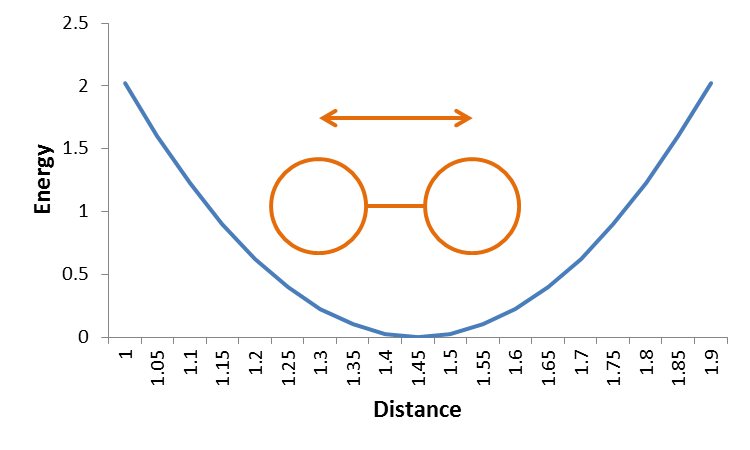
\includegraphics{bond_stretch.png}}
 \caption{Harmonic potential used to describe bonds}\label{fig:bond_stretch}
 \end{center}
\end{figure}

The third term on the right hand side of equation \ref{eq:FF_functional_form} describes the dihedral angles.  $k_\phi$ is the force constant, $n$ controls how many peaks present within the potential (the multiplicity) and $\delta$ shifts the potential to the left or right (the phase).

\begin{figure}[ht]
\begin{center}
 \scalebox{0.6}{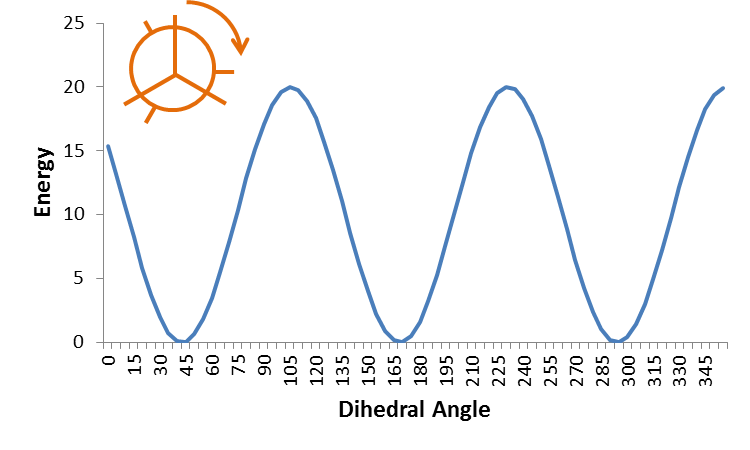
\includegraphics{dihedral_angle.png}}
 \caption{Potential used to describe dihedral angles}\label{fig:dihedral_angle}
 \end{center}
\end{figure}

The last term in equation \ref{eq:FF_functional_form} describes the nonbonding terms and are summed over all non-bonded pairs.  The term is commonly split into two parts, the electrostatics and the dispersion.  The electrostatic interactions are modelled using Coulomb's law,

\begin{equation}
\ U_{elec}=\sum_{i=1}^{N} \sum_{j=1}^{N-1} \frac{q_i q_j}{4 \pi \epsilon_0 r_{ij}} \\.
\end{equation}

Where $q_i$ is the charge on atom $i$, $r_{ij}$ is the distance between atom $i$ and $j$, $N$ is the total number of atoms present and $\epsilon_0$ is the dielectric constant.

If electrostatics were the only interaction considered, atoms with opposing partial charges would be attracted to unrealistically small distances.  By including Van der Waals forces, the attraction caused by the partial charges at small distances is less than the repulsive force considered for the dispersion interactions.  A Lennard-Jones potential is commonly used to describe dispersion,

\begin{equation}
\ U_{disp} = \sum_{i=1}^{N} \sum_{j=1}^{N-1} 4 \epsilon \left[ \left( \frac{\sigma_{ij}}{r_{ij}} \right)^{12} - \left( \frac{\sigma_{ij}}{r_{ij}} \right)^6  \right] \\.
\end{equation}

Where $\epsilon$ is the well depth, $\sigma_{ij}$ is the Lennard-Jones sphere and is related to the position of the minimum $r^*_{ij}$ by the following \cite{cramer_chem},

\begin{equation}
\ r^*_{ij}=2^{1/6} \sigma_{ij} \\.
\end{equation}

$(\sigma/r)^{12}$ described the repulsive dispersion forces and $(\sigma/r)^{6}$ describes the attractive forces.


\begin{figure}[ht]
\begin{center}
 \scalebox{0.6}{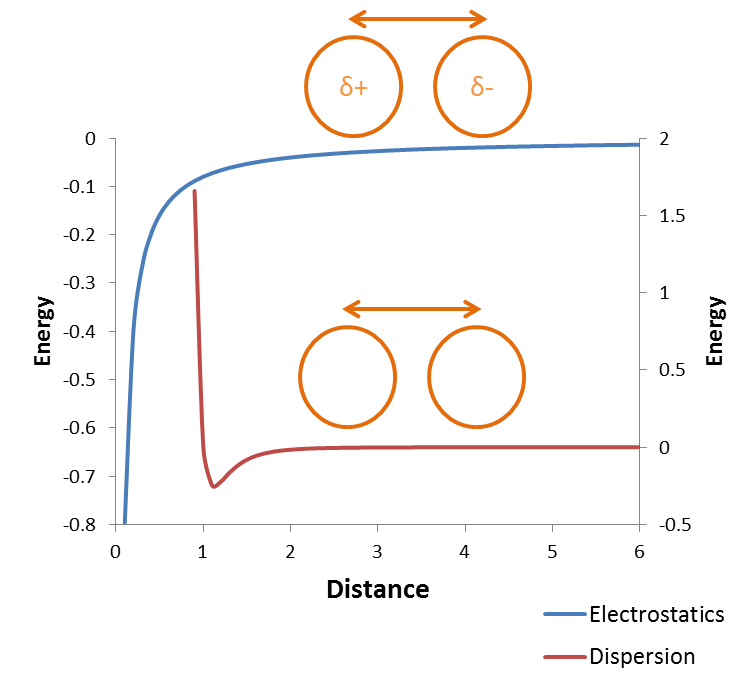
\includegraphics{non-bonded_forces.png}}
 \caption{Potentials used to describe nonbonded interactions, where the right side Energy is the dispersion energy and the left side is the electrostatic energy}\label{fig:non-bonded_forces}
 \end{center}
\end{figure}

Figure \ref{fig:non-bonded_forces} shows that the dispersion forces converge to 0 rapidly compared to the electrostatic forces, which do not converge to 0 within the range of the figure.  The nonbonded forces are the most computationally expensive calculation within the classical potential energy.  To lower this cost, long-range methods are used to calculate these interactions after a cut off distance.  It is common to only calculate the interactions explicitly within a user-defined cut off. However, this cut off is unphysical, so not possible within experiment and changing it can have serious implications for the overall energy of the system \cite{long_range_vdw}.

Within AMBER, Van der Waals interactions are calculated using the following \cite{long_range_vdw},

\begin{equation}
 U_{full}=U_{r<r_c}+U_{r>r_c} \\.
\end{equation}

Where $r$ is the distance between two particles, $r_c$ is the cutoff distance and therefore $U_{r<r_c}$ are the short-range van der Waal interactions.  The long-range interactions, are calculated using the following potential \cite{long_range_vdw},

\begin{eqnarray}
 \ U_{r>r_c} &=& \frac{N\rho}{2}\frac{1}{N(N-1)}\sum_{i<j}^{n}\int_{r_c}^{\infty} 4\epsilon \left[ \left( \frac{\sigma_{ij}}{r} \right)^{12}-\left(\frac{\sigma_{ij}}{r} \right)^{6} \right]g(r)4\pi r^2 dr \nonumber \\ \nonumber
\ & = & 2\pi N \rho \int_{r_c}^{\infty} \left( \langle 4 \epsilon_{ij}\sigma_{ij}^{12}\rangle r^{-12}-\langle 4 \epsilon_{ij}\sigma_{ij}^{6}\rangle r^{-6} \right)r^2 dr \\
\ & = & 8 \pi N \rho \left[ \frac{1}{9}\langle \epsilon_{ij}\sigma^{12}_{ij}\rangle r_{c}^{-9}-\frac{1}{3}\langle \epsilon_{ij}\sigma^{6}_{ij}\rangle r_{c}^{-3} \right] .
\end{eqnarray}

Where $N$ is the total number of particles within the system, $\rho$ is the average density of the system, $\epsilon$ is the well depth, $\sigma_{ij}$ is the Lennard-Jones characteristic radius and $g(r)$ is the radial distribution function which is assumed to be equal to one outside the cutoff distance.  

Long-range van der Waals energies scale to $r^{-6}$, so are small in comparison to long-range electrostatic interactions.  There are many methods currently available to handle long-range electrostatic interactions.  These include the Ewald summation, particle-mesh ewald, reaction field and isotropic periodic sum.

One approach to long range electrostatic interactions is the direct sum approach.  By using a sufficiently large cutoff so that the change in energy would be negligible by increasing the cutoff, each interaction can be calculated explicitly.  In order to achieve this convergence, the cutoff must be very large, a method that is computationally very expensive.  An alternative way is to make use of the the Ewald Summation \cite{ewald_summation_orig}.

\subsection{Ewald Summation}

By splitting the electrostatic interactions of a periodic system into two parts, a short-range and a long-range part, the computational time required can be significantly reduced.  This is possible due to the following relationship,

\begin{equation} \label{eq:relationship_ewald}
 \ \frac{1}{r}=\frac{f(r)}{r}-\frac{1-f(r)}{r} \\.
\end{equation}

When an appropriate choice for $f(r)$ is used, it will handle the rapid variance at short distances and the slow decay at large distances\cite{leach_molecular_modelling}.


\begin{figure}[ht]
\begin{center}
 \scalebox{0.6}{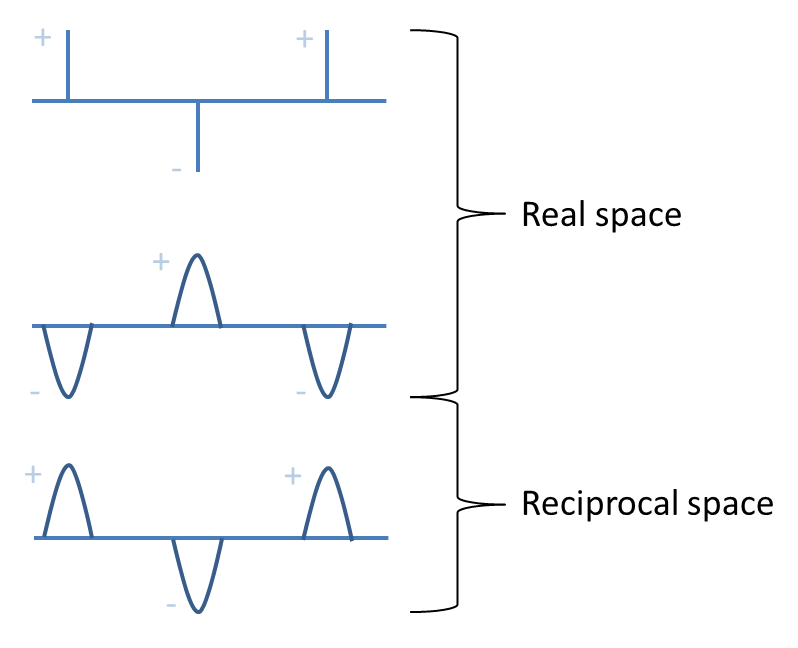
\includegraphics{ewald.png}}
 \caption{Gaussian distributions of equal and opposite charge added to the real space term, then corrected in the reciprocal space term by adding Gaussians of the correct charge.}\label{fig:ewald}
 \end{center}
\end{figure}

The Ewald summation ensures that no long-range interactions are considered for the short-range part of the sum by masking the charges with Gaussian distributions of equal magnitude, but opposite charge.  

The Ewald Summation masks the charges with a Gaussian distribution of equal magnitude, but with opposite charge.  This is illustrated in figure \ref{fig:ewald}.  The short-range calculation (which includes the interaction between charges and the charge distributions used to neutralise them) is then performed by \cite{ewald_help},

\begin{equation}
 \ V_{r<r_c}=\frac{1}{8\pi \epsilon_0}\sum_{|\textbf{n}|=0}^\prime \sum_{i=1}^{N} \sum_{j=1}^{N} \frac{q_iq_jerfc(\alpha|\textbf{r}_{ij}+\textbf{n}|)}{|\textbf{r}_{ij}+\textbf{n}|} \\.
\end{equation}

Where $\alpha$ controls the width of the Gaussians used to mask the charges and is directly related to the cutoff distance, commonly by $\alpha=3.5/r_c$\cite{Stat_mech}, and $\textbf{n}$ is a lattice translation and the prime on the summation indicates that the self interaction, when $i=j$ is not included for the lattice box $|\textbf{n}|=0$.  $erfc(x)$ is the complementary error function,

\begin{equation}
 \ erfc(x)=\frac{2}{\sqrt{\pi}}\int_{x}^{\infty}e^{-t^2}dt \\.
\end{equation}

The long-range calculation must then cancel out the Gaussian distributions used in the short-range calculations, this calculation will not converge in real space\cite{ewald_help}, and as such is performed in reciprocal space using the following sum \cite{leach_molecular_modelling},

\begin{equation}
 \ V_{r>r_c}=\frac{1}{8\pi\epsilon_0} \sum_{k\neq0}\sum_{i=0}^{N}\sum_{j=0}^{N}\frac{1}{\pi L^3}\frac{q_iq_j4\pi^2}{k^2}e^{-k^2/4\alpha^2}\cos(\textbf{k}\cdot \textbf{r}_{ij}) \\.
\end{equation}

Where $\textbf{k}$ are vectors in reciprocal space and are defined as $\textbf{k}=2\pi\textbf{n}/L$.  This long-range sum corresponds to $f(r)$ and $erfc(x)$ corresponds to $1-f(r)$ shown in equation \ref{eq:relationship_ewald}.  In order to cancel out the self interactions that are calculated as a by-product of the long-range sum, an additional term is subtracted to the equation.

\begin{equation}
 \ V_{self}=-\frac{\alpha}{\sqrt{\pi}}\sum_{k=1}^{N}\frac{q_k^2}{4\pi\epsilon_0}
\end{equation}

If the simulation box is surrounded by an infinite medium with a dielectric constant then no further corrections are needed, however, if the surrounding medium is a vacuum, then an additional correction is needed.

\begin{equation}
 \ V_{correction}=\frac{2\pi}{3L^3}\left| \sum_{i=1}^{N}\frac{q_i}{4\pi\epsilon_0} \textbf{r}_i \right|^2 \\.
\end{equation}


The total Ewald summation is then,

\begin{eqnarray}
 \ V_{electrostatic}&=&\frac{1}{8\pi \epsilon_0}\sum_{|\textbf{n}|=0}^\prime \sum_{i=1}^{N} \sum_{j=1}^{N} \frac{q_iq_jerfc(\alpha|\textbf{r}_{ij}+\textbf{n}|)}{|\textbf{r}_{ij}+\textbf{n}|} \nonumber \\
&&+\frac{1}{8\pi\epsilon_0} \sum_{k\neq0}\sum_{i=0}^{N}\sum_{j=0}^{N}\frac{1}{\pi L^3}\frac{q_iq_j4\pi^2}{k^2}e^{-k^2/4\alpha^2}\cos(\textbf{k}\cdot\textbf{r}_{ij}) \nonumber \\
&& -\frac{\alpha}{\sqrt{\pi}}\sum_{k=1}^{N}\frac{q_k^2}{4\pi\epsilon_0}+\frac{2\pi}{3L^3}\left| \sum_{i=1}^{N}\frac{q_i}{4\pi\epsilon_0} \textbf{r}_i \right|^2 .
\end{eqnarray}


\subsection{Particle Mesh Ewald}

The use of the Ewald summation to calculate long-range interactions scales as $N^2$ with the number of charges $N$ \cite{berendsen}.  For this reason, as the system size becomes larger it becomes unsuitable to use.  Approximate methods were therefore developed, one such method is particle mesh Ewald (PME) \cite{PME}.  PME deals with the long range interactions by using fast Fourier transforms (FFTs).  These require spatial points to be interpolated onto a grid or mesh of density values.  The potential can then be solved by using the Poisson equation.  This scales much more favourable at $N\cdot \log (N)$.

\subsection{Solvation models}

Simulating the effect solvent has on a system can be vital to obtaining accurate systematic information.  It is therefore important to consider this when calculating energies and running simulations.  Two methods exist to take account of the interactions between water and solute.  These are explicit and implicit, both are covered briefly here.

\subsubsection{Explicit solvation}

There are three common descriptions used for water models: the 3-site, 4-site and 5-site.  These are illustrated in figure \ref{fig:water_model}.  


\begin{figure}[ht]
\begin{center}
 \scalebox{0.6}{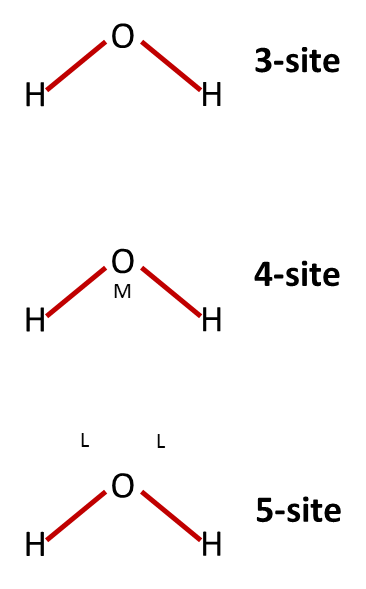
\includegraphics{water_model.png}}
 \caption{The common models used for water.  3-site, 4-site and 5-site differ by the different number of interaction sites.}\label{fig:water_model}
 \end{center}
\end{figure}

As expected, as the number of interaction sites increases the number of calculations required are increased.  The 3-site model is the most simple and has only three points of interaction, where the charges and Lennard-Jones spheres are centred on the atoms.  The 4-site moves the negative charge present on the oxygen closer to the hydrogen atoms (position M), leaving the Lennard-Jones sphere centred on the oxygen.  The 5-site moves the negative charge to represent the lone pairs.

Several examples are shown in table \ref{table:water_parameters} along with the parameters used within equation \ref{eq:FF_functional_form}.  In order to lower the computational cost when explicit water is used, it is common to freeze the bonds, such that the degrees of freedom are lowered to translational and rotational.

\begin{center}
\begin{table*}[ht]
{
\caption{Water parameters used for common water models.}
\hfill{}
\begin{tabular}{c | c | c | c | c}
\hline 
 & SPC \cite{SPC} & TIP3P \cite{tip4p} & TIP4P \cite{tip4p} & TIP5P \cite{tip5p} \\
\hline
r$_{OH}$ (\AA{}) & 1.0000 & 0.9572 & 0.9572 & 0.9572 \\
\hline 
$\theta_{HOH}$ & 109.47 & 104.52 & 104.52 & 104.52 \\
\hline
A $\times$ 10$^{-3}$ (kcal \AA{}$^{12}$/mol) & 629.4 & 582.0 & 600.0 & 544.5 \\
\hline
C (kcal\AA{}$^{6}$/mol) & 625.5 & 595.0 & 610.0 & 590.3 \\
\hline
q$_{O}$ (e) & -0.820 & -0.834 & -1.040 & -0.241 \\
\hline 
q$_{H}$ (e) & 0.410 & 0.417 & 0.520 & 0.241 \\
\hline
r$_{OM}$ (\AA{}) & - & - & 0.15 & - \\
\hline
r$_{OL}$ (\AA{}) & - & - & - & 0.7 \\
\hline
$\theta_{LOL}$ & - & - & - & 109.47 \\
\hline
\end{tabular}}
\hfill{}
\label{table:water_parameters}
\end{table*}
\end{center}


\subsubsection{Implicit Solvation}

Implicit solvation attempts to calculate the effects water has on a solute without calculating the movement occurring within the solvent.

Classical mechanics uses Coulomb's law to describe electrostatics,

\begin{equation}
\ E(\mathbf{r} )=k q_1 \frac{\mathbf{r} - \mathbf{s}}{\vert \mathbf{r} - \mathbf{s} \vert^3} \\.
\end{equation}
%
$E(\mathbf{r})$ is an electric field and $q_1$ is a point charge. $\mathbf{r}$ and $\mathbf{s}$ represent positions in space.  If there are multiple charges a charge density can be used \cite{classical_electrodynamics_book}.

\begin{equation} \label{eq:coulomb_charge_density}
\ E(\mathbf{r} )=k \int \rho(\mathbf{s}) \frac{\mathbf{r} - \mathbf{s}}{\vert \mathbf{r} - \mathbf{s} \vert^3} d^3 \mathbf{s} \\.
\end{equation}
%
Where $\rho(\mathbf{s})$ is the free charge density (the bound charge density relates to polarisation).  Calculating the divergence\footnote{Divergence is a measure of how much the velocity increases in an outward motion, it is the volume density of the outward flux} of both sides of equation \ref{eq:coulomb_charge_density} with respect to $\mathbf{r}$ yields,

\begin{eqnarray}
\ \nabla \cdot E(\mathbf{r}) &=& \nabla \cdot k \int  \rho(\mathbf{s}) \frac{\mathbf{r} - \mathbf{s}}{\vert \mathbf{r} - \mathbf{s} \vert^3} d^3 \mathbf{s} \\
\ &=& k \int \rho(\mathbf{s}) \nabla \cdot \frac{\mathbf{r} - \mathbf{s}}{\vert \mathbf{r} - \mathbf{s} \vert^3} d^3 \mathbf{s} .
\end{eqnarray}

The divergence of the following function has special properties,

\begin{equation}
\ \nabla \cdot \frac{\mathbf{r} - \mathbf{s}}{\vert \mathbf{r} - \mathbf{s} \vert^3} \\.
\end{equation}
%
It should have a large positive divergence, instead it is zero everywhere except the origin.  However, if integrated the result is $4\pi$ if the origin is within the integrated space.  This is very similar to a dirac delta function $\delta ( \mathbf{r} - \mathbf{s})$ \cite{intro_electrodynamics_book}.  The divergence of the electric field is then,

\begin{equation}
\ \nabla \cdot E(\mathbf{r} )=k 4 \pi \int \rho(\mathbf{s}) \delta ( \mathbf{r} - \mathbf{s}) d^3 \mathbf{s} \\.
\end{equation}

Then using the sifting property of a dirac delta function and using $k=1/4\pi \epsilon_0$,

\begin{equation}
\ \nabla \cdot E(\mathbf{r} )=\frac{1}{\epsilon_0} \rho(\mathbf{r}) \\.
\end{equation}
%
Where $\epsilon_0$ is the permittivity of free space\footnote{This is a measure of how much resistance is present when an electric field is formed}.  This relates the charge density to the electric field and is known as Gauss's law.

The electric field $E(\mathbf{r})$ can be written as the gradient of a potental $\phi(\mathbf{r})$,

\begin{eqnarray}
\ E(\mathbf{r}) &=& - \nabla \phi(\mathbf{r}) \\ \label{eq:poisson_equation}
\ \nabla^2 \phi(\mathbf{r}) &=& - \frac{\rho(\mathbf{r})}{\epsilon_0} .
\end{eqnarray}

Equation \ref{eq:poisson_equation} shows the Poisson equation.  If the charge density follows a Boltzmann distribution, the Poisson-Boltzmann equation must be used\cite{Simulate_Phys_world}.  In order to move from the Poisson equation to the Poisson-Boltzmann equation, assume that the concentration $c_i(\mathbf{r})$ of species $i$ with bulk concentration $c_i^0$ at position $\mathbf{r}$ can be calculated by the following Boltzmann distribution,

\begin{equation}
\ c_i (\mathbf{r}) = c_i^0 \exp \left( - \frac{z_ie \phi(\mathbf{r})}{k_BT}  \right) \\.
\end{equation}
%
Where $z_ie$ is the charge of species $i$.  The free charge density can be given by,

\begin{equation}
\ \rho(\mathbf{r}) = F \sum_i c_i^0 z_i \\.
\end{equation}
%
Where $F$ is the Faraday constant.  Putting this back into the Poisson equation, we obtain the Poisson-Boltzmann equation,

\begin{equation} \label{eq:Poisson_boltzmann}
\ \nabla^2 \phi(\mathbf{r}) = - \frac{F}{\epsilon_0} \sum_i c_i^0 z_i \exp \left( - \frac{z_ie \phi(\mathbf{r})}{k_BT}  \right) \\.
\end{equation}

In order to solve equation \ref{eq:Poisson_boltzmann}, numerical approaches are applied.  One such method is finite difference.  A grid is superimposed onto the system and each grid point is assigned a value for the charge density, electrostatic potential, ionic strength and dielectric constant \cite{Leach_chem}.  The derivatives required for equation \ref{eq:Poisson_boltzmann} are then calculated using finite difference.  Each grid point has an effect on its surrounding points, thus this is an iterative process.

The non-polar interactions are then approximated, these include the cavity energy and the Van der Waals energy.  The cavity energy is the energy required to make a cavity in a water box, and the Van der Waals energy is the interaction between the protein and the surrounding water.  These tend to be parametrised using experimental values \cite{Leach_chem}.


\subsection{Force fields}

This section so far has dealt with functional forms, solvation and how long range forces are dealt with.  The equations require parameters in order to calculate energies.  These parameters are based on values obtained from \textit{ab initio} methods and experimental data and collected together in force fields.  Some example force fields that are available in AMBER\cite{amber_ref} are listed below.

\noindent
\textbf{ff94}\cite{ff94}

Charges are based on multiple-conformation HF/6-31G* calculations, the forcefield was developed for use with proteins.

\noindent
\textbf{ff96}\cite{ff96}

Modified the backbone parameters of the ff94.

\noindent
\textbf{ff99}\cite{ff99}

Small changes to the protein parameters implemented.

\noindent
\textbf{ff99SB}\cite{amber_ff_review}

New parameters for the backbone dihedral angles.

\noindent
\textbf{ff14SB}\cite{amber14}

Improvements to the side chain and backbone parameters.

\noindent
\textbf{GAFF}\cite{gaff}

Generalised amber force field, designed to be used with small organic molecules.

\clearpage
%%%%%%%%%%%%%%%%%%%%%%%%%%%%%%%%%%%%%%%%%%%%%%%%%%%%%%%%%%%%%%%%%%
%%%%%%%%%%%%%%%%%%%%%%%%%%%%%%%%%%%%%%%%%%%%%%%%%%%%%%%%%%%%%%%%%%
%%%%%%%%%%%%%%%%%%%%%%%%%%%%%%%%%%%%%%%%%%%%%%%%%%%%%%%%%%%%%%%%%%
%%%%%%%%%%%%%%%%%%%%%%%%%%%%%%%%%%%%%%%%%%%%%%%%%%%%%%%%%%%%%%%%%%

\section{Quantum Mechanics}

Quantum Mechanics describes the behaviour of subatomic particles.  Within chemistry, the most applicable of these is the electron.  The classical description of atoms acting as hard spheres bonded together by springs is rethought and a new quantum description of particles is used.  In the quantum world, particles have the qualities typical of both solid matter and waves and are described by a wavefunction.  This wave-particle duality was suggested by Louis de Broglie \cite{DeBroglie_thesis} when he showed that the momentum of a particle is inversely proportional to the wavelength,

\begin{equation}
\ p = \frac{h}{\lambda} \\.
\end{equation}
%
Where $p$ is the momentum, $\lambda$ is the wavelength and $h$ is Plank's constant \cite{Planck}.

To take measurements of the position of an electron, a very small wavelength must be used, but short wavelengths are very high in energy $E$,

\begin{equation}
\ E= \frac{hc}{\lambda} \\.
\end{equation}

Using a high energy beam will have a consequence, the momentum will be altered.  This is Heisenberg's uncertainty principle\cite{Heisenberg}, the more accurately the position is known the less accurately the momentum can be known.

\begin{equation}
\ \Delta x \Delta p \geq \frac{h}{4 \pi} \\.
\end{equation} 
%
$\Delta x$ is the uncertainty on the position and $\Delta p$ the uncertainty in the momentum.  $\frac{h}{4 \pi}$ is the limit that the position and momentum can be known.

\subsection{The wavefunction $\Psi$}

A position of an electron can never be known exactly, so probabilities are used instead.  If a region of space has a high probability of finding an electron, then the electron density is high\cite{chemical_bonding}.  In order to obtain any physically relevant information from a wavefunction, the use of operators is required. By using the relevant operator on a wavefunction, any observable can be obtained.  To obtain real-valued eigenvalues, the operators need to be Hermitian, such that\cite{susskind_quantum},

\begin{equation}
\ \langle A | \hat{O} | B \rangle = \langle B | \hat{O} | A \rangle^* \\.
\end{equation}

Where the superscript $*$ represents the complex conjugate.  Additionally the electron density can be obtained from the wavefunction $\psi$ by multiplication with its complex conjugate.

The time independent Schr\"odinger equation\cite{Schrodinger} is used to obtain the energy of the wavefunction using the Hamiltonian operator \^H, it is impossible to solve completely except for the most simple cases.

\begin{equation}
\ \hat{H} \psi = E \psi \\.
\end{equation}
%
Where $E$ is the energy eigenvalue of the system, $\psi$ is the eigenfunction and the Hamiltonian (\^H) can be split into the operator for the kinetic energy \^T and the potential energy \^V.

\begin{eqnarray}
\hat{H} &=& \hat{V} + \hat{T} \\
\ &=& \hat{V}_{NN} \lbrace R \rbrace + \hat{V}_{Ne}\lbrace R;r \rbrace + \hat{V}_{ee} \lbrace r \rbrace + \hat{T}_N \lbrace R \rbrace + \hat{T}_e\lbrace r \rbrace \label{eq:pre_BO}
\end{eqnarray}
%
Where $\hat{V}_{NN} \lbrace R \rbrace$ is the nuclear-nuclear repulsion, $\hat{V}_{Ne}\lbrace R;r \rbrace$ is the nuclear-electron attraction, $\hat{V}_{ee} \lbrace r \rbrace$ is the electron-electron repulsion, $\hat{T}_N \lbrace R \rbrace$ is the kinetic energy of the nuclei and $\hat{T}_e\lbrace r \rbrace$ is the kinetic energy of the electrons.  These can be further subdivided into,


\begin{eqnarray} \label{eq:full_hamiltonian}
\hat{H} &=& \frac{1}{2} \sum_{k=1}^{N} \sum_{l\neq k}^{N} \frac{Z_k Z_l e^2}{4 \pi \epsilon_0 R_{kl}} 
+ \sum_{i=1}^{n} \sum_{k= 1}^{N} \frac{Z_k e^2}{4 \pi \epsilon_0 R_{ik}} \nonumber \\
& & + \frac{1}{2} \sum_{i=1}^{n} \sum_{j\neq i}^{n} \frac{e^2}{4 \pi \epsilon_0 r_{ij}} 
- \frac{\hbar}{2} \sum \frac{\nabla^2_{R_k}}{m_n} - \frac{\hbar}{2} \sum \frac{\nabla^2_{r_i}}{m_e} .
\end{eqnarray}
%
Where $Z_k$ is the atomic charge on atom $k$, $R_{kl}$ is the distance between atom $k$ and $l$, $N$ is the number of atoms, $n$ is the number of electrons, subscript $i$ and $j$ are electrons and $e$ is the elementary charge.  $\nabla^2$ is the Laplacian operator and in a three dimensional cartesian frame takes the form,

\begin{equation}
\ \nabla^2 = \frac{\partial^2}{\partial x_i^2} + \frac{\partial^2}{\partial y_i^2} + \frac{\partial^2}{\partial z_i^2} \\.
\end{equation}


\subsection{Born-Oppenheimer Approximation}

Equation \ref{eq:pre_BO} can be simplified by using the Born-Oppenheimer approximation\cite{Born-Oppenheimer}.  The mass of protons and neutrons are around 1800 times that of the mass of electrons\cite{cramer_chem} and it can therefore be approximated that electrons move much faster than the protons and neutrons.  If taking this approximation into account the electrons can be thought to rearrange themselves instantaneously  to any nuclear movement.  Equation \ref{eq:pre_BO} can then be simplified to,

\begin{equation}
\ \hat{H}_{elec} = \hat{V}_{Ne}\lbrace R;r \rbrace + \hat{V}_{ee} \lbrace r \rbrace + \hat{T}_e\lbrace r \rbrace \\.
\end{equation}
%
Where the nuclear kinetic energy can now be ignored, the nuclear-nuclear repulsion is constant and the nuclear-electron attraction can be thought of as an external potential acting on the electrons.  $\hat{H}_{elec}$ is the electronic Hamiltonian, which makes up the electronic Schr\"odinger equation,

\begin{equation} \label{eq:electronic_schrodinger}
\ \hat{H}_{elec} \psi_{elec} = E_{elec} \psi_{elec} \\.
\end{equation}


\subsection{Potential Energy Surfaces}

Without the Born-Oppenheimer approximation, the notion of a potential energy surface could not exist.  Potential energy surfaces are utilised a great deal in the field of computational chemistry, as they provide a relationship between the energy and geometry of a system.  By changing the nuclear coordinates and calculating the electronic energy, these surfaces can show where any minima or transition states are.  Figure \ref{fig:PES} shows an example potential energy surface for the C-O bond and the C-O-H angle with a fixed dihedral angle in methanol.

\begin{figure}[ht]
\begin{center}
 \scalebox{0.8}{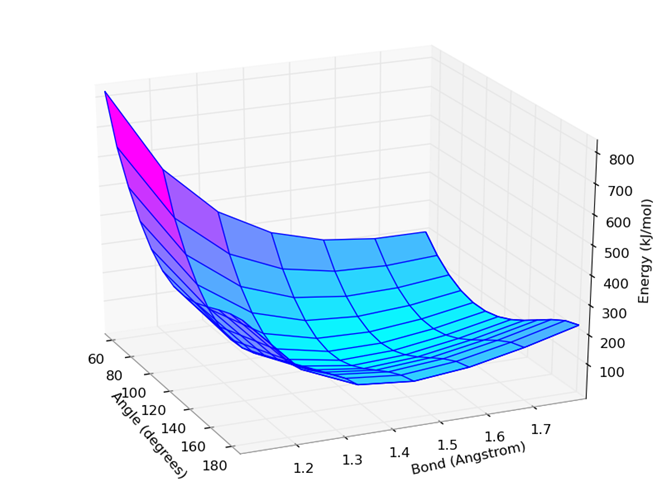
\includegraphics{QM_PES_methanol.png}}
 \caption{Potential Energy surface for 2 degrees of freedom in methanol}\label{fig:PES}
 \end{center}
\end{figure}

In order to construct a potential energy surface, after equation \ref{eq:electronic_schrodinger} has been solved an additional term must be included to account for the nuclear-nuclear repulsion,

\begin{equation}
\ E_{PES} = E_{elec} + \sum^N_{k=1} \sum^N_{l\neq 1} \frac{Z_{k}Z_{l}}{|\mathbf{R}_k - \mathbf{R}_l |} \\.
\end{equation}


\subsection{The Variational Principle} \label{sec:variational}

The variational principle will provide an approximation to the ground state energy by combining orthonormal wavefunctions.  Wavefunctions can be combined into a single trial function by a linear combination of wave functions with weighting coefficients.

\begin{equation}
\Phi=\sum_{\alpha} c_{\alpha} \Phi_{\alpha}
\end{equation}

Where orthonormal wavefunctions are orthogonal such that $\int \psi_{i} \psi_{j} d \mathbf{r} = 0$ if $i\neq j$ and normalised, $\int \psi_{i}^2 d \mathbf{r} =1$.

This trial function must be subject to the same boundary conditions as the wave functions and $\sum_{\alpha}|c_{\alpha}|^2=1$.  The variational principle states that the energy obtained from a trial function will be greater than or equal to the true ground state energy\cite{levine_quantum}.

\begin{equation}
\ \langle \Phi | H | \Phi \rangle \ge E_0
\end{equation}

An approximation to the ground state energy is found by minimising the energy with respect to the weighting coefficients.  Proof of the theorem can be seen below\cite{Szabo_quantum}.

\begin{eqnarray}
\ \langle \Phi | \Phi \rangle &=& 1 \label{eq:var1} \\
\ \sum_{\alpha} | \Phi_{\alpha} \rangle \langle \Phi_{\alpha} | &=&1 \label{eq:var2} \\
\ \langle \Phi_{\alpha} | \Phi_{\beta} \rangle &=& \delta_{\alpha \beta} \label{eq:var3} \\
\  \langle \Phi | \Phi \rangle &=& \sum_{\alpha \beta} \langle \Phi | \Phi_{\alpha} \rangle \langle \Phi_{\alpha} | \Phi_{\beta} \rangle \langle \Phi_{\beta} | \Phi \rangle \nonumber \\
\ &=& \sum_{\alpha \beta}  \langle \Phi | \Phi_{\alpha} \rangle \delta_{\alpha \beta}  \langle \Phi_{\beta} | \Phi \rangle \nonumber \\
\ &=& \sum_{\alpha} \langle \Phi | \Phi_{\alpha} \rangle \langle \Phi_{\alpha} | \Phi \rangle \nonumber \\
\ &=& \sum_{\alpha} | \langle \Phi_{\alpha} | \Phi \rangle |^2 \label{eq:var4} \\
\ \langle \Phi | H | \Phi \rangle &=& \sum_{\alpha \beta} \langle \Phi | \Phi_{\alpha} \rangle \langle \Phi_{\alpha} | H | \Phi_{\beta} \rangle \langle \Phi_{\beta} | \Phi \rangle \nonumber \\
\ &=& \sum_{\alpha}E_{\alpha} | \langle \Phi_{\alpha} | \Phi \rangle |^2 \label{eq:var5} .
\end{eqnarray}

Since $E_{\alpha}\ge E_0$,

\begin{eqnarray}
\ \langle \Phi | H | \Phi \rangle &\ge& \sum_{\alpha} E_0 | \langle \Phi_{\alpha} | \Phi \rangle |^2 \nonumber \\
\ &\ge& E_0 \sum_{\alpha} | \langle \Phi_{\alpha} | \Phi \rangle |^2 \nonumber \\
\ &\ge& E_0 .
\end{eqnarray}

Where equations \ref{eq:var1}, \ref{eq:var2} and \ref{eq:var3} are true due to the orthonormality of wave functions and in equation \ref{eq:var5} equation \ref{eq:var4} has been applied.

\subsection{Hartree-Fock}

The Hartree-Fock approximation (HF) provides a method to solve the electronic Schr\"odinger equation (equation \ref{eq:electronic_schrodinger}).  It deals with the many electron problem as many one-electron problems with an average electron-electron repulsion acting on each electron.  It is because of this that it is sometimes referred to as ``mean-field theory''.  Each electron occupies a spin orbital $\chi(\mathbf{x})$, which is a molecular orbital $\psi(\mathbf{r})$ with spin coordinates (either $\alpha(\omega)$ or $\beta(\omega)$)\cite{skylaris_lecture}.  The Pauli exclusion principle states that the wavefunction must change sign if two electrons are swapped within the system\cite{OCP_comp_chem}, such that $\Psi(\mathbf{x}_1, \mathbf{x}_2)$ = $-\Psi(\mathbf{x}_2, \mathbf{x}_1)$.  This anti-symmetric behaviour is upheld within HF by the introduction of Slater determinants.  For example, a two electron system would have the following determinant,

\begin{equation}
\Psi(\mathbf{x}_1, \mathbf{x}_2) = \sqrt{\frac{1}{2!}}
	\begin{bmatrix}
		\chi_1(\mathbf{x}_1) & \chi_2(\mathbf{x}_1) \\
		\chi_1(\mathbf{x}_2) & \chi_2(\mathbf{x}_2) \\
	\end{bmatrix}
\end{equation}

\begin{equation}
\ \Psi(\mathbf{x}_1, \mathbf{x}_2) = \sqrt{\frac{1}{2!}} ( \chi_1(\mathbf{x}_1)\chi_2(\mathbf{x}_2) - \chi_2(\mathbf{x}_1)\chi_1(\mathbf{x}_2)) \\.
\end{equation}

If the electrons change place, the determinant then becomes,

\begin{eqnarray}
\ \Psi(\mathbf{x}_2, \mathbf{x}_1) &=& \sqrt{\frac{1}{2!}} ( \chi_1(\mathbf{x}_2)\chi_2(\mathbf{x}_1) - \chi_2(\mathbf{x}_2)\chi_1(\mathbf{x}_1)) \\
\ \therefore \Psi(\mathbf{x}_1, \mathbf{x}_2) &=& -\Psi(\mathbf{r}_2, \mathbf{r}_1) .
\end{eqnarray}

The single electron problem with average electron-electron repulsion is expressed within the Fock operator, 

\begin{eqnarray}
\ \hat{f}_i &=& -  \frac{1}{2} \hat{\nabla}^2_i - \sum_{k=1}^{N_{atoms}} \frac{Z_{k}}{\mathbf{R}_{ik}} + \hat{v}_{i} \\
\ &=& \hat{h}_i + \hat{v}_{i} .
\end{eqnarray}
%
Where $\hat{v}_{i}$ is the average potential felt by electron $i$ due to all other electrons.  This energy can be divided into the Coulombic and exchange energies, shown in equation \ref{eq:coulomb} and \ref{eq:exchange} respectively.

\begin{eqnarray}
\ J_{ij} &=& \int \int \chi_{i}^{*}(\mathbf{x}_1) \chi_{j}^{*}(\mathbf{x}_2) \frac{1}{r_{ij}} \chi_{i}(\mathbf{x}_1) \chi_{j}(\mathbf{x}_2) d\mathbf{x}_1 d\mathbf{x}_2 \label{eq:coulomb}\\
\ K_{ij} &=& \int \int \chi_{i}^{*}(\mathbf{x}_1) \chi_{j}^{*}(\mathbf{x}_2) \frac{1}{r_{ij}} \chi_{j}(\mathbf{x}_1) \chi_{i}(\mathbf{x}_2) d(\mathbf{x}_1) d(\mathbf{x}_2)\label{eq:exchange}
\end{eqnarray}

The exchange operator is present because of the asymmetric nature of the wavefunction, which is another consequence of the Pauli exclusion principle, stating that no two electrons can have the same quantum number.

The Fock operator can then be written as,

\begin{equation}
\ \hat{f}_i = \hat{h}_i + \sum_{j}^{n/2} (2J_j(\mathbf{r}_i) - K_j(\mathbf{r}_i)) \\.
\end{equation}

The energy of the system is obtained self-consistently as the Fock operator depends on the molecular orbitals that we are trying to calculate.  This process is shown in figure \ref{fig:HF_flowchart}.

\begin{figure}[ht]
\begin{center}
 \scalebox{0.9}{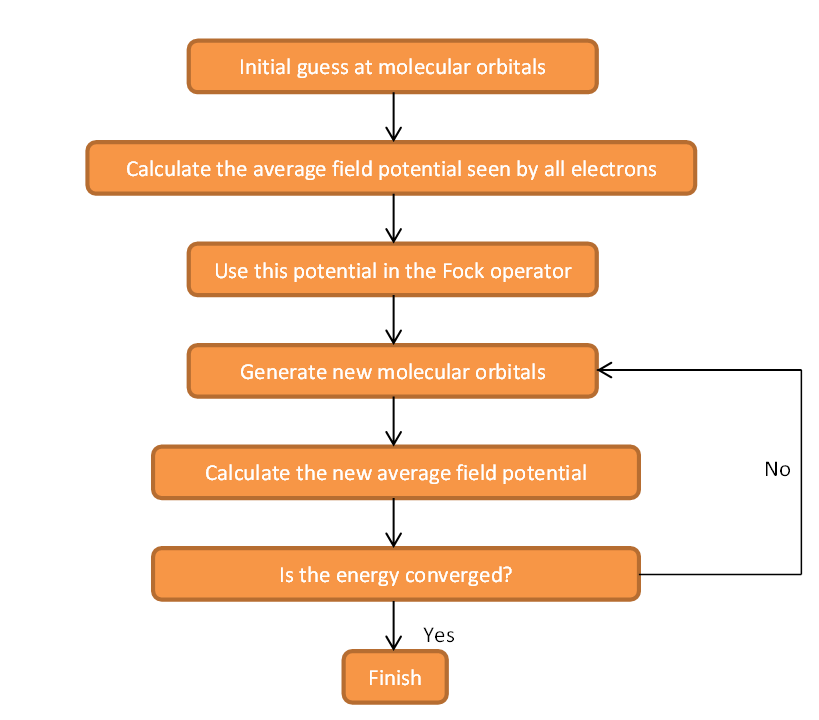
\includegraphics{Flow_chart_HF_1.png}}
 \caption{The SCF process used within the HF approximation}\label{fig:HF_flowchart}
 \end{center}
\end{figure}

As described in section \ref{sec:variational} (The Variational Principle), the energy is minimised to the lowest possible value $E_{HF}$.  The difference between $E_{HF}$ and the ground state energy, $E_{0}$ is known as the correlation energy.

\pagebreak
\subsection{Density Functional Theory}

In contrast to wavefunction approaches, like HF, density functional theory (DFT) uses the electronic density to calculate the energy.  By using the density instead of the wavefunction, the cost of any calculations is limited: for an $n$ electron system, the wavefuntion becomes a 3$n$-dimensional quantity, whereas the density remains 3-dimensional.  This lower cost makes DFT very computationally appealing and explains its rise in popularity.  As previously mentioned, to get properties from the wavefunction operators are used, to get properties from the density, however, functionals must be used\footnote{A functional swallows a function to produce a number}.  Hohenberg and Kohn\cite{Hohenburg_Kohn} state that all ground state electronic properties can be obtained from the density of the system in this manner.

\subsubsection{Hohenberg and Kohn's first theorem}

The first theorem states that the external potential $v_{ext}$ is determined by the ground state density \cite{Hohenburg_Kohn, DFT_intro_Harrison}.  This statement can be proved by \textit{reductio ad absurdum}. 

Assume that there are two external potentials that provide the same density $n(\mathbf{r})$, but have different ground states $\Psi_1$ and $\Psi_2$.  So for each ground state, we have Hamiltonian $\hat{H}_1$ and $\hat{H}_2$ and ground state energy $E_1$ and $E_2$ with external potentials $v_{ext, 1}$ and $v_{ext, 2}$.  Then including the variational principle, the following is true,

\begin{eqnarray}
\ E_2 &=& \langle \Psi_2 | \hat{H}_2 | \Psi_2 \rangle < \langle \Psi_1 | \hat{H}_2 | \Psi_1 \rangle \\
\ &=& \langle \Psi_1 | \hat{H}_1 | \Psi_1 \rangle + \langle \Psi_1 | \hat{H}_2 - \hat{H}_1 | \Psi_1 \rangle \\ \label{eq:HK1_1}
\ E_2 &<& E_1 + \int [v_{ext, 2} (\mathbf{r}) - v_{ext, 1} (\mathbf{r})]n(\mathbf{r})d\mathbf{r} .
\end{eqnarray}

Similarly for $E_1$,

\begin{eqnarray}
\ E_1 &=& \langle \Psi_1 | \hat{H}_1 | \Psi_1 \rangle < \langle \Psi_2 | \hat{H}_1 | \Psi_2 \rangle \\
\ &=& \langle \Psi_2 | \hat{H}_2 | \Psi_2 \rangle + \langle \Psi_2 | \hat{H}_1 - \hat{H}_2 | \Psi_2 \rangle \\ \label{eq:HK1_2}
\ E_1 &<& E_2 + \int [v_{ext, 1} (\mathbf{r}) - v_{ext, 2} (\mathbf{r})]n(\mathbf{r})d\mathbf{r} .
\end{eqnarray}

Combining equation \ref{eq:HK1_1} and \ref{eq:HK1_2} gives,

\begin{equation}
\ E_2 + E_1 < E_1 + E_2 \\.
\end{equation}

Which is a nonsensical equation and therefore proves that only one external potential exists for the density.

\subsubsection{Hohenberg and Kohn's second theorem}

As $\Psi$ is a functional of $n(\mathbf{r})$, then the kinetic and electron-electron interaction operators must be also.  Therefore, a universal functional ($F[n(\mathbf{r})]$) can be defined that is not dependent on the number of particles and is valid for any external potential,

\begin{eqnarray}
\ F[n(\mathbf{r})] &=& \langle \Psi | \hat{T}+\hat{V}_{ee} | \Psi \rangle \\ \label{eq:HK2_1}
\ E[n(\mathbf{r})] &=& \int v_{ext}(\mathbf{r}) n(\mathbf{r})d \mathbf{r} + F[n(\mathbf{r})] .
\end{eqnarray}

Examination of equation \ref{eq:HK2_1} shows that for the correct density, the ground state energy can be found, which is the focus of the second theorem.  To prove this, consider the following energy,

\begin{equation}
\ E [\Psi'] = \langle \Psi' | \hat{V}_{ext} | \Psi' \rangle + \langle \Psi' | \hat{T}+ \hat{V}_{ee} | \Psi' \rangle \\,
\end{equation}

has a minimum at the ground state energy.  Therefore,

\begin{eqnarray}
\ E [\Psi'] &=& \int v_{ext}(\mathbf{r}) n'(\mathbf{r}) d \mathbf{r} + F[n'(\mathbf{r})] \\
\ E [\Psi] &=& \int v_{ext}(\mathbf{r}) n(\mathbf{r}) d \mathbf{r} + F[n(\mathbf{r})] \\
\ E [\Psi] &<& E [\Psi'] .
\end{eqnarray}

If $F[n(\mathbf{r})]$ were known exactly, then the calculation of the ground state energy would be trivial, however, determination of the universal function is highly non-trivial.

\subsubsection{Kohn-Sham Theory}

The current popularity of DFT is largely down to the Kohn-Sham\cite{Kohn_Sham} reformulation.  The issue of finding a universal function is dealt with by representing the ground state density with the density of a system of non-interacting electrons $n_s(\mathbf{r})$.  The energy is then found using the following,

\begin{equation} \label{eq:KS0}
\ E[n_s] = T_s[n_s] + U[n_s] + V_{ext}[n_s] + E_{xc}[n_s] \\.
\end{equation}
%
Where $T_s[n_s]$ is the kinetic energy for non-interacting electrons, $U[n_s]$ is the Coulomb energy given by the Fock equation, $V_{ext}[n_s]$ is the external potential, $E_{xc}[n_s]$ is known as the exchange correlation functional and can be split into the kinetic correlation energy, $T_c[n_s]$, and the exchange energy $V_{ee}[n_s]$.

$E_{xc}[n_s]$ is used to correct for the fact that a non-interacting system has been used,

\begin{eqnarray}
\ E_{xc}[n_s] &=& T_c[n_s] + V_{ee}[n_s] \\
\ T_c[n_s] &=& T[n_0] - T_s[n_s] \\
\ V_{ee}[n_s] &=& V_{ee}[n_0] - U[n_s] \label{eq:KS1} .
\end{eqnarray}

The exchange energy is a completely non-classical term caused by the exchange of two same spin electrons.  Equation \ref{eq:KS0} can be written in terms of Kohn-Sham orbitals,

\begin{eqnarray}
\ E[n_s] &=& \sum_{i=1}^{n} 
\int \chi_{i}^{*}(\mathbf{r}) \left[ - \frac{1}{2} \nabla^2 \right] \chi_{i}(\mathbf{r}) d \mathbf{r} \nonumber \\
 &-& \sum_{i=1}^{n} \sum_{k=1}^{N} \int  \chi_{i}^{*}(\mathbf{r}) \left[ \frac{Z_k}{|\mathbf{r}_i - \mathbf{R}_k |}  \right] \chi_{i}(\mathbf{r}) d \mathbf{r} \nonumber \\
  &+& \sum_{i=1}^{n} \int \chi_{i}^{*}(\mathbf{r}) \left[ \frac{1}{2} \int \frac{n_s}{| \mathbf{r}_i - \mathbf{r}_j | }d(\mathbf{r}_j) \right] \chi_{i}(\mathbf{r}) d \mathbf{r} + E_{xc}[n_s] . \label{eq:KS2}
\end{eqnarray}

No term exists for the exchange-correlation functional, if there was then Kohn-Sham theory would be exact. 

\subsubsection{Exchange-Correlation Functional}

The importance of the exchange-correlation term within Kohn-Sham DFT is highlighted above.  It is common practice to separate this functional into the exchange term and the correlation term,

\begin{equation}
\ E_{xc}[n_s] = E_x [n_s] E_c[n_s] \\.
\end{equation}

These components can then be treated as individual entities.  Some approximations used to calculate the exchange-correlation energy are described in the next two sections.


\textbf{Local Density Approximation}

The simplest method to calculate the exchange-correlation energy is the local density approximation (LDA).  The exchange energy is calculated within LDA by using the local density of a region and creating a uniform electron gas with the same density.  The exchange energy is then calculated for this fictitious system using the following,

\begin{equation}
\ E^{LDA}_{x}[n_s] = - \frac{3}{4} \left( \frac{3}{\pi} \right)^{\frac{1}{3}} \int n_{s}(\mathbf{r})^{\frac{4}{3}} d \mathbf{r} \\.
\end{equation}

No equivalent term exists for the correlation energy\cite{cramer_chem}.  However, the correlation energy has been calculated using quantum Monte Carlo techniques and, by using a suitable analytical interpolation formula, the energy can be matched\cite{jensen_quantum}.  Such methods are used within the VWN (Vosko, Wilk and Nusair)\cite{VMN_LDA} functional.

LDA works well for systems with uniform density.  However, molecules show a cusp in density around nuclei, and because of this, LDA is not a suitable method for use with molecules.

\textbf{Generalised Gradient Approximation}

The generalised gradient approximation (GGA) uses the value from LDA and adds a correctional term to take into account the gradient of the density.  The exchange-correlation energy then takes the following form,

\begin{equation}
\ E^{GGA}_{x}[n_s(\mathbf{r})] = E^{LDA}_{x}[n_s(\mathbf{r})] + \Delta E_{x}\left[ \frac{| \nabla n_s(\mathbf{r}) |}{n_s(\mathbf{r})^{\frac{4}{3}}} \right] \\.
\end{equation}

The first exchange functional was developed by Beck (B88)\cite{B88_GGA}, 

\begin{equation} \label{eq:XC1}
\ E^{GGA}_{x}[n_s(\mathbf{r})] = E^{LDA}_{x}[n_s(\mathbf{r})] + E^{B88}_{x}[n_s(\mathbf{r})] \\.
\end{equation}

Many functionals were developed based on the B88, where no empirical data is used and everything is calculated from first principles.  One example of this, which is used throughout this thesis is the PBE functional\cite{GGA_made_simple}.

The correlation energy is also improved within GGA.  Some functionals correct the LDA correlation energy, in a similar manner to equation \ref{eq:XC1}, like the PW91 functional\cite{PW91}.  The LYP (Lee, Yang and Parr) functional\cite{LYP} calculates the correlation energy by empirical fitting based on simulations performed on the helium atom.

In practice GGA functionals fit within two distinct categories,

\begin{description}
  \item[First] Those that are fitted based on experimental data.
  \item[Second] Those that are calculated explicitly in each simulation.
\end{description}

\subsubsection{Basis Sets}

The wavefunction has an unknown functional form, so in practice it is made up of many known functions, a basis set.  This is not an approximation: in the event of an infinite basis set, any other functions can be made.  When considering computational effort, however, an infinite basis set is infeasible.  So, as is so common within computational chemistry, a compromise must be made between the computational time and accuracy for any calculation.  As such, the development of more accurate basis sets has three goals \cite{cramer_chem},

\begin{description}
  \item[first] minimise the number of basis functions,
  \item[second] be chosen such that integration can be completed in an efficient manner,
  \item[third] be large in the same regions that the probability density is large.
\end{description}

\textbf{Slater-Type orbitals}

In 1930 Slater introduced Slater-type orbitals \cite{STO}.  These functions exponentially decay at long range and show a cusp at the nucleus which is exact for the hydrogen atom.  However, no radial nodes exist within an STO, so these are made by linear combination of many STOs \cite{jensen_quantum}.  The functional form can be seen below,

\begin{equation}
\ \chi_{\zeta,n,l,m}(r, \theta, \varphi)= N Y_{l,m}(\theta, \varphi)r^{n-1}e^{-\zeta r} \\.
\end{equation}

Where $N$ is a normalisation constant, $Y_{l,m}$ are spherical harmonic functions, $n$ is the principle quantum number, $r$ is the distance of the electron from the nucleus and $\zeta$ is a constant relating to the effective charge of the nucleus.  Figure \ref{fig:STO} shows an example Slater-Type orbital.


\begin{figure}[ht]
\begin{center}
 \scalebox{0.9}{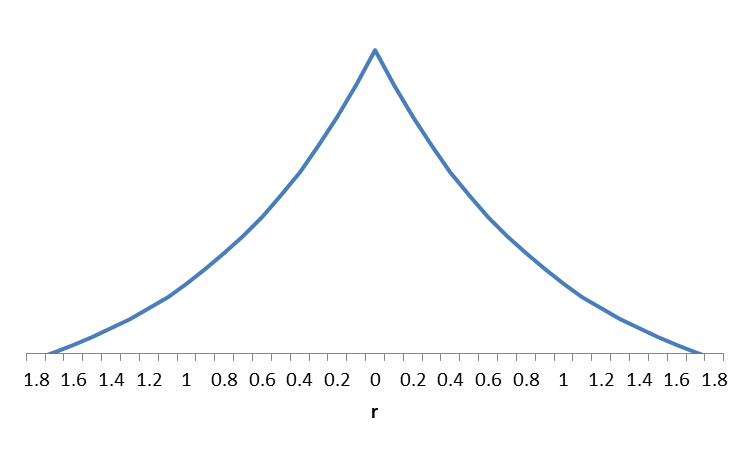
\includegraphics{STO.png}}
 \caption{Slater-Type orbital}\label{fig:STO}
 \end{center}
\end{figure}

The disadvantage with STOs is that there is no analytical solution to the two electron mutli-centred integrals, meaning these have to be computed numerically.  This is computationally costly, thus the use of STOs is limited to small systems.

\textbf{Gaussian-Type orbitals}

In 1950 Boys introduced a new type of orbital that has an analytical solution to the multi-centred integrals \cite{Boys_GTO}.  This new orbital changed the $e^r$ term within the STO functional form to $e^{r^2}$, which provides a Gaussian distribution.  The functional form then becomes simply,

\begin{equation}
\ \chi_{\zeta,n,l,m}(r, \theta, \varphi)= N Y_{l,m}(\theta, \varphi)r^{n-1}e^{-\zeta r^2} \\.
\end{equation}

However, an individual (or primitive) Gaussian provides a poor representation of the orbital, so multiple Gaussians are combined by linear combination (contracted Gaussians).  Using this process, more complex shapes can be formed and orbitals are better represented.  The orbitals are then represented by,

\begin{equation}
\  \chi_{\zeta,n,l,m}(r, \theta, \varphi)=\sum_{\alpha=1}^{M} C_{\alpha} N Y_{l,m}(\theta, \varphi)r^{n-1}e^{-\zeta r^2} \\.
\end{equation}

The number of primitive Gaussians used within contracted Gaussians can be controlled to balance the computational accuracy with efficiency.  Commonly, a split valence is used, this occurs when a different number of primitive Gaussians have been used to describe the core and valence electrons.  For example the 3-21G basis set uses 3 primitives within a contracted Gaussian to describe core electrons and two contracted Gaussians, one with 2 primitive Gaussians and one with 1 primitive, to describe the valence electrons.

\textbf{Basis Set Superposition Error}

Using GTO or STO to calculate the interaction energy of a system ($\Delta E = E_{COMPLEX} - E_{HOST} - E_{LIGAND}$) or any atom centred basis set, will result in basis set superposition error (BSSE).  The error arises from an overlap of the basis set in the complex, i.e. the basis function centred on the ligand overlaps with the host.  This effect is not duplicated when calculating either the host or ligand in the absence of the other, which will overestimate interaction energies.  One way of solving this issue is the introduction of ghost atoms within the host and ligand calculations, so the basis functions are still available to overlap.

\textbf{Plane Wave Basis Sets}

In contrast to the previously mentioned basis sets, the plane wave basis is centred in space and not on atoms.  Because of this it does not not suffer from BSSE, however, the box size will have an effect on the speed of the calculation.  Plane waves are used when periodic boundaries must be present within the simulation and are the solution to the periodic Schr\"{o}dinger equation.  The form of a plane wave for a cubic box with side length $l$ is,

\begin{eqnarray}
\ \psi_{\mathbf{k}}(\mathbf{r}) &=& \frac{1}{l^{\frac{3}{2}}} e ^{i(k_x x+k_y y + k_z z)} \\
\ &=& \frac{1}{V^{\frac{1}{2}}} e^{i \mathbf{k}\cdot\mathbf{r}} .
\end{eqnarray}

Where $k_x =  \frac{2\pi}{l}n_x$ and $n_x, n_y, n_z \in \mathbb{Z}$.\footnote{Where $\mathbb{Z}$ is a set of integers and $\in$ means ``is an element of''}  Plane waves are distributed evenly over a grid within the box and because of this cannot accurately represent the electrons tightly bound around the nucleus, so are used primarily to describe the valence density.  To overcome this ``effective core potentials" (ECP) or pseudopotentials are commonly used to describe the behaviour of the core electrons.

\textbf{Pseudopotentials}

In 1934 Hans G. A. Hellmann introduced the pseudopotential \cite{pseudopotential_intro}.  The use of a pseudopotential eliminates the need for core electrons to be described by a basis set, and instead uses an effective potential.  Using this potential makes the approximation that the core electrons can be considered, along with the nucleus, as rigid and non-polarisable.  Without the use of pseudopotentials, basis sets such as the plane wave basis sets would be far too computationally expensive to be useful.  This is because of the rapid oscillations of the wavefunction at small distances from the nucleus.

When deriving suitable pseudopotentials, it is required that the energy and magnitude of the potential be the same after a cut off $r_c$.  For soft pseudopotentials, this cut off is large, which leads to faster convergence, but makes the pseudopotential less transferable.  

\begin{figure}[ht]
\begin{center}
 \scalebox{0.9}{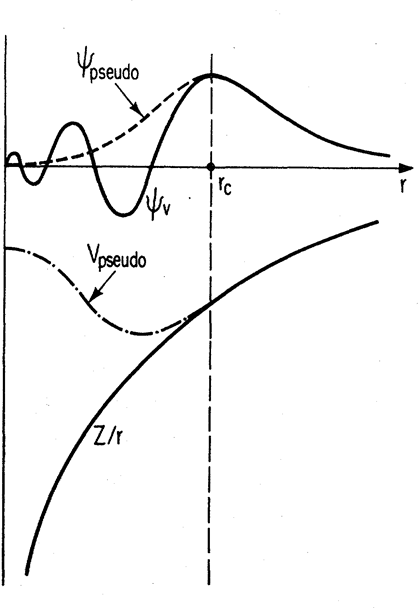
\includegraphics{pseudopotential.png}}
 \caption{Pseudopotential (dashed line) with an all electron potential (solid line), taken from reference \cite{PP_image}}\label{fig:PP}
 \end{center}
\end{figure}

\subsubsection{ONETEP}

ONETEP (Order-N Electronic Total Energy Program) can perform DFT calculations on thousands of atoms by making use of linear scaling DFT methods.  As previously mentioned, DFT methods scale by $\mathcal{O}(N^3)$ where N is the number of electrons present within a system.  This restriction means that traditional DFT can only be performed on relatively small systems.  Linear scaling DFT, however, makes use of the exponential decay of the density matrix for systems with a bandgap\cite{exp_decay}.  In practice this is done by applying a cutoff within the single particle density matrix $\rho(\mathbf{r}, \mathbf{r}^{\prime})$, where the single particle density matrix is formed by,

\begin{equation}
\ \rho(\mathbf{r}, \mathbf{r}^{\prime}) = \sum_{n} | \psi_{n}(\mathbf{r}) \rangle f_n \langle \psi_n (\mathbf{r}^{\prime}) |
\end{equation}


Where $f_n$ is the occupation number.  The diagonal of the density matrix provides the density, and within traditional DFT methods this is evaluated by direct diagonalisation of the Hamiltonian.  For large systems this is not feasible, so a cutoff is applied to the density matrix based on distance $| \mathbf{r} - \mathbf{r}^{\prime}|$.  A decrease in this cutoff will increase the speed of the calculation, but lower the accuracy.

Within ONETEP, the density matrix is written as,

\begin{equation}
\ \rho(\mathbf{r}, \mathbf{r}^\prime) = \sum_{\alpha \beta}\phi_\alpha (\mathbf{r}) K^{\alpha \beta} \phi^{*}_{\beta}( \mathbf{r}^{\prime}) \\.
\end{equation}

Where ${\phi_{\alpha}(\mathbf{r})}$ are a set of spatially localised non-orthogonal generalised Wannier functions\cite{NGWF} (NGWFs), an example of which is shown in figure \ref{fig:NGWF}.  $K^{\alpha \beta}$ is the density Kernel\cite{Density_Kernel}, which is the representation of the density matrix in a set of duals of the NGWFs, and a generalisation of the occupation numbers $f_n$ to nonorthogonal functions.


\begin{figure}[ht]
\begin{center}
 \scalebox{0.4}{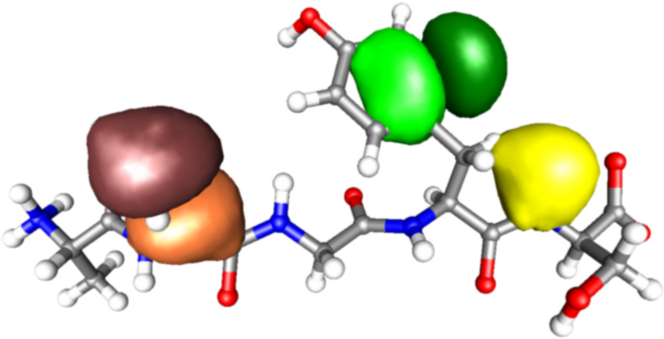
\includegraphics{NGWF_example.png}}
 \caption{Three NGWFs on an oligopeptide, taken from \cite{onetep_website}}\label{fig:NGWF}
 \end{center}
\end{figure}

Linear scaling is achieved within ONETEP by applying a cutoff, as described above, to the density kernel and by strict localisation of the NGWFs to atomic centres.  ONETEP operates by employing a nested loop, an outer loop which controls the optimisation of the NGWFs and an inner loop which controls the optimisation of the density kernel.  The loops continue in a self consistent manner until convergence has been achieved.  Once the NGWFs have been optimised, they contain the same information as the Kohn-Sham orbitals of the system and because they are optimised \textit{in situ} they alter to their chemical environment.  Similarities are present between the combination of the NGWFs and the combination of delocalised orbitals within traditional cubic scaling DFT up to the boundary of the NGWF.  Therefore by altering the radii of the NGWF, the same accuracy as cubic scaling DFT can be achieved.  This comparable accuracy is shown in reference \cite{ONETEP}.

The optimisation procedure of the NGWFs is performed by expansion in a psinc (periodic cardinal sine) basis\cite{Psinc}.  Psinc functions are related to plane waves by Fourier transform and are highly localised and orthogonal by nature.  Each psinc function is centered on a grid point and therefore the basis set can be controlled by changing the spacing between each point.  An example of a pisnc function is shown in figure \ref{fig:psinc_function}.

\begin{figure}[ht]
\begin{center}
 \scalebox{0.8}{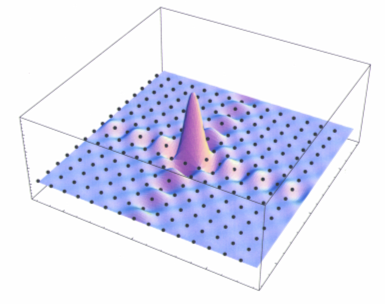
\includegraphics{psinc_function.png}}
 \caption{A psinc function taken from reference \cite{psinc_pic}}\label{fig:psinc_function}
 \end{center}
\end{figure}

In a similar manner to a plane wave basis, because a psinc basis is not atomic centred, ONETEP does not suffer from BSSE.

The attractive dispersion forces present within systems are not explicitly calculated by DFT.  As such an empirical correction is applied within ONETEP\cite{dispersion_onetep} in a similar fashion to the DFT+D approach described by Grimmer et al.\cite{Grimmer}.  These corrections include the Elstner\cite{Elstner} and Grimme D2\cite{Grimmer} and are parameterised for specific functionals.


%Match Order N^3
%Expanded in a psinc basis
%What is a psinc basis set
%No BSSE
%parallelised to run on thousands of atoms

\clearpage
%%%%%%%%%%%%%%%%%%%%%%%%%%%%%%%%%%%%%%%%%%%%%%%%%%%%%%%%%%%%%%%%%%
%%%%%%%%%%%%%%%%%%%%%%%%%%%%%%%%%%%%%%%%%%%%%%%%%%%%%%%%%%%%%%%%%%
%%%%%%%%%%%%%%%%%%%%%%%%%%%%%%%%%%%%%%%%%%%%%%%%%%%%%%%%%%%%%%%%%%
%%%%%%%%%%%%%%%%%%%%%%%%%%%%%%%%%%%%%%%%%%%%%%%%%%%%%%%%%%%%%%%%%%

\section{Molecular Dynamics} \label{sec:molecular_dynamics}

The previous sections explained how the energy of a stationary molecule can be calculated.  However, the most interesting properties of molecules comes from an average of many structures.  As such, methods exist to accurately generate an ensemble of structures.  One of these methods, molecular dynamics (MD) \cite{MD_original}, achieves this by calculating the motion of a molecule when forces are applied to it \cite{OCP_comp_chem}.  If the ergodic hypothesis is satisfied, i.e. the average properties obtained from the system over time are the same as the average properties over the whole statistical ensemble, then accurate macroscopic thermodynamic properties can be calculated \cite{McQuarrie_stat_mech}.

Newton's second law (equation \ref{eq:newton_second_law}) describes the relationship between the force $\mathbf{F}_i$ and acceleration $\mathbf{a}_i$ of a particle with mass $m_i$.  By integrating this equation and with knowledge of the forces applied, the positions of the atoms can be found.

\begin{eqnarray} \label{eq:newton_second_law}
\ \mathbf{F}_i &=& m_i \mathbf{a}_i \\
\ \label{eq:newton_second_law_vel} &=& m_i \frac{d \mathbf{v}_i}{dt} \\
\ \label{eq:newton_second_law_pos} &=& m_i \frac{d^2 \mathbf{r}_i}{dt^2} .
\end{eqnarray}

Equations \ref{eq:newton_second_law_vel} and \ref{eq:newton_second_law_pos} use the relationship between the acceleration and velocity $v_i$ and the position $\mathbf{r}_i$ respectively.  The force can also be calculated from the gradient of the potential energy,

\begin{equation} \label{eq:newton_force_energy}
\ \mathbf{F}_i = - \nabla_i U \\.
\end{equation}

Combination of equation \ref{eq:newton_second_law_pos} and \ref{eq:newton_force_energy} yields a relationship between the potential energy and position of the atoms at time $t$,

\begin{equation}
\ - \frac{d U}{d \mathbf{r}_i} = m_i \frac{d^2 \mathbf{r}_i}{dt^2} \\.
\end{equation}

The simplest application is to assume that the acceleration is a constant.  Using this assumption the velocities and positions can be found simply by integrating the following equations with respect to time,

\begin{eqnarray}
\ \mathbf{a}_i &=& \frac{d \mathbf{v}_i}{dt} \\
\ \mathbf{v}_i &=& \frac{d \mathbf{r}_i}{dt} .
\end{eqnarray}

Which gives respectively,

\begin{eqnarray} \label{eq:vel_accel}
\ \mathbf{v}_i &=& \mathbf{a}_i t + \mathbf{v_0}_i \\ \label{eq:pos_vel}
\ \mathbf{r}_i &=& \mathbf{v}_i t + \mathbf{r_0}_i .
\end{eqnarray}

The combination of equation \ref{eq:vel_accel} and \ref{eq:pos_vel} gives,

\begin{equation} \label{eq:euler}
\ \mathbf{r}_i = \mathbf{a}_i t^2 + \mathbf{v_0}_i t + \mathbf{r_0}_i \\.
\end{equation}

The initial velocities are often chosen from a Gaussian distribution, with the following functional form,

\begin{equation} \label{eq:kinetic_energy_gaussian}
\ E_{KIN} = \prod_{i=1}^{n} \frac{\sqrt{m_i}}{\sqrt{2\pi k_B T}} \exp \left[ - \beta \frac{\mathbf{p}^2_{i}}{2m_i}  \right] \\.
\end{equation}

This is identical to a selection using a Maxwell-Boltzmann distribution.  In order to clarify this, we must start at the Boltzmann distribution of the kinetic energy,

\begin{equation}
\ \rho(E_{KIN}) = \exp [ -\beta E_{KIN} ] \\.
\end{equation}

Where $\rho(E_{KIN})$ is the probability of kinetic energy $E_{KIN}$.  From here we can derive both the Maxwell-Boltzmann distribution.  By splitting the kinetic energy into the $x$, $y$ and $z$ components we obtain,

\begin{equation}
\ E_{KIN} = \frac{1}{2m}p_{x}^2 + \frac{1}{2m}p_{y}^2 + \frac{1}{2m}p_{z}^2 \\.
\end{equation}

 This is then put back into equation \ref{eq:kinetic_energy_gaussian}.  The Maxwell-Boltzmann distribution then provides us with the probability a molecule will have velocity between $v_x$ and $v_x + dv_x$, $v_y$ and $v_y + dv_y$, $v_z and v_z + dv_z$, summing these together will give the probability that a molecule will have velocity between $v$ and $v+dv$.  This forms a spherical shell of thickness dv, the volume of this shell is $4\pi \mathbf{v}^2$.  If this is placed back into the Gaussian distribution the Maxwell-Boltzmann distribution is achieved.
 
\begin{equation}
 \ E_{KIN} = \prod_{i=1}^{n} 4\pi \left( \frac{m}{2\pi k_B T} \right)^{3/2} \mathbf{v}^2 \exp \left[ - \frac{\beta m \mathbf{v}^2}{2}  \right] \\.
\end{equation}

\subsection{Integration Algorithms}

Direct application of equation \ref{eq:euler} is numerically unstable for all but the most simplistic systems.  As such integration algorithms exist with the following aims:

\begin{itemize}
\item Energy and momentum must be conserved
\item Computational efficiency
\item Long time steps.
\end{itemize}

Three integrators that are commonly used are the Verlet, velocity-Verlet and leapfrog algorithms.  All of which use Taylor expansions to solve the equations of motion.

\begin{eqnarray} \label{eq:Taylor_forward}
\ \mathbf{r}(t+ \delta t) &=& \mathbf{r}(t) + \mathbf{v}(t) \delta t + \frac{1}{2} \mathbf{a}(t) \delta t^2 + \cdots \\
\ \mathbf{v}(t+ \delta t) &=& \mathbf{v}(t) + \mathbf{a}(t) \delta t + \frac{1}{2} \mathbf{b}(t) \delta t^2 + \cdots \\
\ \mathbf{a}(t+\delta t) &=& \mathbf{a}(t) + \mathbf{b}(t) \delta t + \cdots .
\end{eqnarray}

Where the velocity $\mathbf{v}(t)$ is the first derivative, the acceleration $\mathbf{a}(t)$ is the second derivative and $\mathbf{b}(t)$ is the third derivative and so on.  The Verlet algorithm \cite{Verlet} uses two Taylor series expansions, one at $t+ \delta t$ and one at $t - \delta t$ .  Where the Taylor series for $t - \delta t$ is shown in equation \ref{eq:Taylor_reverse} and the combination of this with equation \ref{eq:Taylor_forward} ($t + \delta t$) is shown in equation \ref{eq:verlet}.

\begin{eqnarray} \label{eq:Taylor_reverse}
\ \mathbf{r}(t- \delta t) &=& \mathbf{r}(t) - \mathbf{v}(t) \delta t + \frac{1}{2} \mathbf{a}(t) \delta t^2 + \cdots \\ \label{eq:verlet}
\ \mathbf{r}(t+ \delta t) &=& 2 \mathbf{r}(t) - \mathbf{r}(t- \delta t) + \mathbf{a} \delta t^2 .
\end{eqnarray}

One should note, however, that velocities are not explicitly calculated using this method.  Therefore, the velocities are calculated by the following,

\begin{equation}
\ \mathbf{v}(t) = \frac{\mathbf{r}(t + \delta t) - \mathbf{r}(t - \delta t)}{2 \delta t} \\.
\end{equation}

In addition to not calculating the velocity explicitly, to calculate the next position $\mathbf{r}(t+\delta t)$ the current and previous positions must be known.  This algorithm was later adapted into the velocity-Verlet algorithm \cite{velocity_verlet}, where the velocities are explicitly calculated.

\begin{eqnarray}
\ \mathbf{r}(t+ \delta t) &=& \mathbf{r}(t) + \mathbf{v}(t) \delta t + \frac{1}{2} \mathbf{a}(t) \delta t^2 \\
\ \mathbf{v}(t+ \delta t) &=& \mathbf{v}(t) + \frac{1}{2}[ \mathbf{a}(t) + \mathbf{a}(t+ \delta t) ] \delta t .
\end{eqnarray}

Another variation based on the Verlet algorithm is the leap-frog algorithm.  Within the leap-frog algorithm the velocities are calculated at half time-steps.

\begin{eqnarray}
\ \mathbf{r}(t + \delta t) &=& \mathbf{r}(t) + \mathbf{v} \left( t + \frac{1}{2} \delta t \right) \delta t \\
\ \mathbf{v} \left( t + \frac{1}{2} \delta t \right) &=& \mathbf{v} \left( t - \frac{1}{2}  \delta t \right) + \mathbf{a} (t) \delta t . 
\end{eqnarray}

\subsection{Ensembles}

Depending on the purpose of the simulation, MD can be performed in a number of statistical ensembles.  Within this thesis only three ensembles are used, the microcanonical (NVE) the canonical (NVT) and the isothermal-isobaric (NPT).  The NVE ensemble is an example of a thermodynamic closed system, no particles or energy are exchanged outside of the system.  The N within NVE stands for constant number of particles, the V for constant volume and the E for constant energy.  The NVT and NPT ensemble are examples of thermodynamic closed systems, energy can be transferred into and out of the system, but the particles can not.  The T in NVT and NPT stands for constant temperature and the P for constant pressure.  

Both NVT and NPT can be thought of as close system within an isolated system, where outside the closed system is a heat bath allowing the flow of heat energy into the system and controlling the temperature.  This is illustrated in figure \ref{fig:ensembles}.

\begin{figure}[ht]
\begin{center}
 \scalebox{0.7}{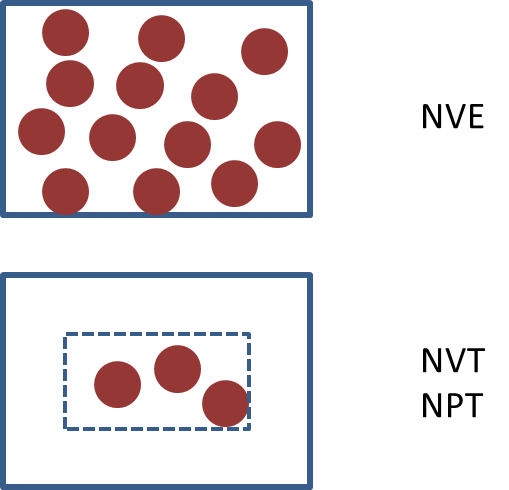
\includegraphics{ensembles.png}}
 \caption{Illustration describing the statistical ensembles, NVE is an isolated system, both NVT and NPT are closed systems within an isolated system}\label{fig:ensembles}
 \end{center}
\end{figure}

Within the NPT and NVT ensembles it is necessary to control the temperature, this is done by use of a thermostat.  Two commonly used examples are the Berendsen \cite{berendsen} and Langevin \cite{langevin} thermostats.  The Berendsen thermostat regulates the temperature by simply scaling the velocities.  The rate in temperature change is given by,

\begin{equation}
\ \frac{d T}{dt} = \frac{1}{\tau} (T_0 - T) \\.
\end{equation}

Where $\tau$ is a time constant and $T_0$ is the target temperature.  The velocities are then scaled, $\mathbf{v}(t)^{\prime} = \lambda \mathbf{v}(t)$, to match the target temperature \cite{Thermostat_lecture}. The Berendsen thermostat is known to have issues with producing correct canonical ensembles for small systems, however, for large system sizes the approximation produces accurate properties \cite{berendsen_weakness}.

The Langevin thermostat controls the temperature by solving the Langevin equations of motion, which differ to the Newton equations by an introduction of a friction constant $\zeta$.  The equations of motion are then,

\begin{equation}
\ m_i \mathbf{a}_i = \mathbf{F}_i + \zeta \mathbf{v}_i + f^{\prime} \\.
\end{equation}

Where $f^{\prime}$ is a random force determined from a Gaussian distribution.

Similarly, within an NPT ensemble the pressure must be regulated too.  This is done by using a barostat.  Pressure can be calculated using the Claussias Virial Theorem \cite{leach_molecular_modelling}, 

\begin{equation}
\ P = \frac{1}{V} \left[ N k_B T - \frac{1}{3} \sum_{i=1}^{N} \sum_{j=i+1}^{N} r_{ij}f_{ij} \right] \\.
\end{equation}

Where $P$ is the pressure, $V$ is the volume, $r_{ij}$ is the distance between particle $i$ and $j$ and $f_{ij}$ is the force acting between those particles.  Within the Berendsen barostat the volume is scaled to adjust the pressure using the scaling parameter $\mu$, in a similar way as within the thermostat \cite{barostat_lecture}.

\begin{equation}
\ \mu = \left[ 1 - \frac{\beta \partial t}{\tau} (P_0 - P) \right]^{\frac{1}{3}} \\.
\end{equation}

Where $\beta$ is the isothermal compressibility and $P_0$ is the target pressure.


\subsection{Time Efficiency}

Running MD simulations on large systems can be costly, because of this many methods exist to lower these costs.  One such method is the application of periodic boundaries, by running a smaller system with periodic boundaries, bulk properties can be calculated.  This is illustrated in figure \ref{fig:periodic_boundaries}.

\begin{figure}[ht]
\begin{center}
 \scalebox{0.7}{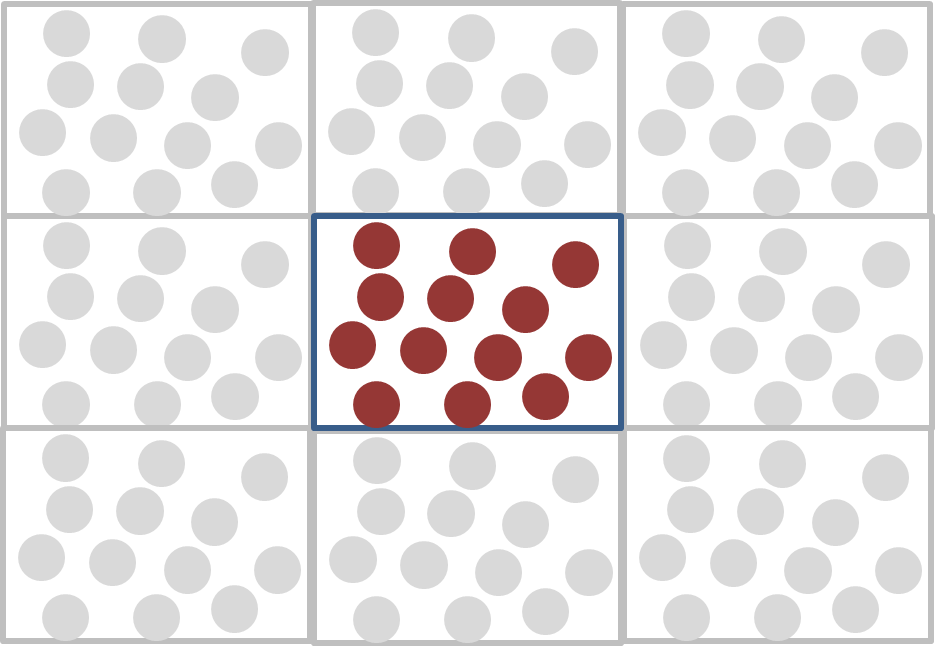
\includegraphics{periodic_boundaries.png}}
 \caption{Illustration describing periodic boundaries, the center box is calculated explictly and the forces from the other boxes are applied to it}\label{fig:periodic_boundaries}
 \end{center}
\end{figure}

In addition, the time step can be increased by freezing out the fastest vibrations, such as bonds involving hydrogen.  Two constraint algorithms that do this were used in this thesis, these were SHAKE \cite{shake} and LINCS \cite{Lincs}.

\clearpage
%%%%%%%%%%%%%%%%%%%%%%%%%%%%%%%%%%%%%%%%%%%%%%%%%%%%%%%%%%%%%%%%%%
%%%%%%%%%%%%%%%%%%%%%%%%%%%%%%%%%%%%%%%%%%%%%%%%%%%%%%%%%%%%%%%%%%
%%%%%%%%%%%%%%%%%%%%%%%%%%%%%%%%%%%%%%%%%%%%%%%%%%%%%%%%%%%%%%%%%%
%%%%%%%%%%%%%%%%%%%%%%%%%%%%%%%%%%%%%%%%%%%%%%%%%%%%%%%%%%%%%%%%%%


\section{Monte Carlo} \label{sec:monte_carlo}

Another way to generate an ensemble of structures is to use Monte Carlo.  Whereas molecular dynamics allows the movement of a system as it evolves through time, Monte Carlo applies random moves and then accepts or rejects them.  As such, it does not require the kinetic energy and so can use the configurational partition function (see section \ref{sec:free_energy} for a definition).  Monte Carlo is a stochastic approach to generating structures, in order to ensure that it remains random (unlike the deterministic approach of MD) a Markov chain is constructed.  Structures are accepted into a Markov chain by comparison with the structure that immediately preceded  it only.

A Markov chain must satisfy the balance condition \cite{comp_sim_liquids_book},

\begin{equation}
\ \sum_{m} \rho_m \pi_{mn} = \rho_n \\.
\end{equation}

When

\begin{equation}
\ \sum_n \pi_{mn}=1 \\.
\end{equation}

Where $\rho$ is the state probability and $\pi$ is the transition probability.  One way to ensure that this is satisfied is to apply the overstrict detailed balance condition,

\begin{equation} \label{eq:detailed_balance}
\ \rho_{m} \pi_{mn} = \rho_{n} \pi_{nm} \\.
\end{equation}

There are two aspects of the transition matrix, the trial probability $t_{mn}$ and the acceptance probability $\pi^{acc}_{mn}$.  The trial probability controls how large the movements are between structures \cite{monte_carlo_note_shell}, for example this could be the displacement of one atom.

Rearranging equation \ref{eq:detailed_balance} gives,

\begin{equation}
\ \frac{\pi_{mn}}{\pi_{nm}} = \frac{\rho_n}{\rho_m} \\.
\end{equation}

Then using the definition of the transition probability,

\begin{equation}
\ \frac{\pi^{acc}_{mn}}{\pi^{acc}_{nm}} = \frac{t_{nm}\rho_n}{t_{mn}\rho_m} \\.
\end{equation}

Where $\rho$ is given by the Boltzmann probability,

\begin{equation}
\ \rho = \frac{\exp - \beta U(\mathbf{r})}{Z(N,V,T)} \\.
\end{equation}

Cancellation of the partition functions leaves

\begin{eqnarray}
\ \frac{\pi^{acc}_{mn}}{\pi^{acc}_{nm}} &=& \frac{\exp[ -\beta U_2 ]}{\exp [- \beta U_1]} \\
\ &=& \exp [ -\beta U_2 + \beta U_1 ] \\
\ &=& \exp [ - \beta ( U_2 - U_1) ]
\end{eqnarray}

When $U_2 < U_1$ then the move will always occur, so a $min$ function can be introduced,

\begin{equation}
\ \pi^{acc}_{mn}= min [ 1, \exp (- \beta (U_2 - U_1)) ] \\.
\end{equation}

This equation is known as the Metropolis-Hastings criterion \cite{metropolis-hastings}.  It can be shown that it satisfies detailed balance \cite{Hammersley_monte_carlo},

\begin{eqnarray}
\ \frac{\pi^{acc}_{mn}}{\pi^{acc}_{nm}} &=& \frac{min[1, \exp ( - \beta (U_2-U_1))]}{min[1, \exp ( - \beta (U_1-U_2))]} \\
 \ &=& \begin{cases} \frac{\exp [ - \beta (U_2-U_1)]}{1} \text{if $U_2 > U_1$} \\ \frac{1}{\exp [ - \beta (U_1-U_2)]} \text{if $U_1 > U_2$} \end{cases} .
\end{eqnarray}




\clearpage
%%%%%%%%%%%%%%%%%%%%%%%%%%%%%%%%%%%%%%%%%%%%%%%%%%%%%%%%%%%%%%%%%%
%%%%%%%%%%%%%%%%%%%%%%%%%%%%%%%%%%%%%%%%%%%%%%%%%%%%%%%%%%%%%%%%%%
%%%%%%%%%%%%%%%%%%%%%%%%%%%%%%%%%%%%%%%%%%%%%%%%%%%%%%%%%%%%%%%%%%
%%%%%%%%%%%%%%%%%%%%%%%%%%%%%%%%%%%%%%%%%%%%%%%%%%%%%%%%%%%%%%%%%%

\section{Free Energy} \label{sec:free_energy}

Free energy is the easiest way to make comparisons directly from theory to experiment. It is is calculated using the rules of statistical mechanics, the object of which is to provide mathematical relations to equilibrium properties of macroscopic systems \cite{intro_stat_thermodynamics}, i.e. it provides the link between what is observed using theoretical methods and what is observed in the macroscopic world.  Statistical mechanics introduces a function that if known, all thermodynamic values (entropy, free energy, temperature etc..) can be exactly calculated \cite{stat_mech_surv_guide}.  This function is known as the partition function and the canonical partition function has the following functional form,

\begin{equation}
\ Q(N,V,T)= \frac{1}{h^{3N}N!}\int \exp(-\beta H(\mathbf{p}, \mathbf{r})) d\mathbf{p} d\mathbf{r} \\.
\end{equation}

To know the value of the partition function requires the knowledge of all energy levels and their occupancy within a system.  The only way to know this is to sample infinitely, which is obviously not feasible.  Because of this relative free energies are commonly calculated, this will be further explained later.

The probability of selecting a structure with energy $H$ is,

\begin{equation}
\ \rho(\mathbf{r}, \mathbf{p}) = \frac{\exp(-\beta H(\mathbf{r}, \mathbf{p})}{Q(N,V,T)} \\.
\end{equation}

For simplicity the kinetic energy part of the Hamiltonian can be integrated out and an analytical formula can be found.

\begin{eqnarray}
\ Q(N,V,T) &=& \frac{1}{h^{3N}N!}\int \exp(-\beta U(\mathbf{r}))d \mathbf{r} \int \exp(-\beta K(\mathbf{p}))d \mathbf{p} \\ \label{eq:kinetic_integration}
\ \int \exp(-\beta K(\mathbf{p}))d \mathbf{p} &=& (2 \pi k_B Tm )^{\frac{3N}{2}} \\
\ Q(N,V,T) &=& \frac{(2 \pi k_B Tm )^{\frac{3N}{2}}}{h^{3N}N!} \int \exp(-\beta U(\mathbf{r}))d \mathbf{r} \\
\ &=& \frac{1}{N!} \left( \frac{2 \pi k_B T m}{h^2} \right)^{\frac{3N}{2}} \int \exp(-\beta U(\mathbf{r}))d \mathbf{r} \\
\ Z(N,V,T) &=& \int \exp(-\beta U(\mathbf{r}))d \mathbf{r} \\
\ Q(N,V,T) &=& \frac{1}{N![\Lambda(T)]^{3N}} Z(N,V,T) .
\end{eqnarray}

Where $\Lambda(T)^{3N}$ is the thermal de Broglie wavelength (the average wavelength of gas particles in an ideal gas at temperature T) and the step in equation \ref{eq:kinetic_integration} is performed using the following,

\begin{eqnarray}
\ \int \exp (-\beta K (\mathbf{p}))d \mathbf{p} &=& \int \exp \left(- \beta \frac{\mathbf{p}^2}{2m} \right) \\
\ y &=& \sqrt{\beta \frac{\mathbf{p}^2}{2m}} \\
\ &=& \left( \frac{\beta}{2m} \right)^{\frac{1}{2}} \mathbf{p} \\
\ \frac{dy}{d\mathbf{p}} &=& \left( \frac{\beta}{2m} \right)^{\frac{1}{2}} \\
\ d\mathbf{p} &=& \frac{dy}{\left( \frac{\beta}{2m} \right)^{\frac{1}{2}}} \\
\ \sqrt{2m k_B T}\int \exp ( -y^2)dy &=& \sqrt{2 \pi m k_B T} .
\end{eqnarray}


 $Z(N,V,T)$ is the configurational partition function, by using this we can calculate the probability of selecting a conformation based on the potential energy.

\begin{equation}
\ \rho(\mathbf{r})= \frac{\exp (-\beta U(\mathbf{r}))}{Z(N,V,T)} \\.
\end{equation}

The knowledge of partition functions and how to use them to obtain probabilities can then be combined to calculate free energies.  As mentioned previously, absolute free energies (free energies relative to an empty cavity) require infinite sampling, because of this relative free energies are commonly calculated.  There are several methods that allow the calculation of relative free energies, two of the most common among these are thermodynamic integration and free energy perturbation.  Both methods have advantages and disadvantages and will be described in more detail.

\subsection{Thermodynamic Integration}

Thermodynamic Integration (TI) introduces a switching function to smoothly move from one state to another.  By using a switching function the degree of overlap between the start and end states is irrelevant as a number of intermediate states are introduced.  These states do not have to have any physical significance and are merely a tool used to smooth the path.  The switching function $\lambda$ is introduced into the partition function,

\begin{equation}
\ Q(N,V,T,\lambda) = \frac{1}{h^{3N}N!}\int \exp(-\beta U(\mathbf{r}, \lambda))d \mathbf{r} \int \exp(-\beta K(\mathbf{p}))d \mathbf{p} \\.
\end{equation}

Where $U(\mathbf{r}, \lambda)$ has the following functional form,

\begin{equation}
\ U(\mathbf{r}, \lambda) = \lambda U_{A}(\mathbf{r})+ (1-\lambda) U_B (\mathbf{r}) \\.
\end{equation}

So when $\lambda=0$ we are sampling from state A an when $\lambda=1$ state B is sampled.  The use of this partition function leads to the following free energy \cite{Stat_mech},

\begin{equation}
\ A(N,V,T,\lambda)=-k_B T \ln Q(N,V,T,\lambda) \\.
\end{equation}

Then, using partial differentiation,

\begin{eqnarray} \label{eq:ti_partial_diff}
\ \frac{ \partial A(N,V,T,\lambda)}{\partial \lambda} &=& - \frac{k_BT}{Q(N,V,T, \lambda)} \frac{\partial Q(N,V,T, \lambda)}{\partial \lambda} \\ \label{eq:ti_partial_diff2}
\ &=& - \frac{k_BT}{Z(N,V,T, \lambda)} \frac{\partial Z(N,V,T, \lambda)}{\partial \lambda} .
\end{eqnarray}

The step in equation \ref{eq:ti_partial_diff} is performed by application of the chain rule, and the step in equation \ref{eq:ti_partial_diff2} comes from analytical integration of the kinetic energy cancelling.  Although this may not be the case if the mutation occurs between different size atoms, if the full free energy cycle is applied the kinetic energy is compensated \cite{Simulate_Phys_world}.

The partial differential of $Z(N,V,T, \lambda)$ is then,

\begin{eqnarray}
\ - \frac{k_BT}{Z(N,V,T, \lambda)} \frac{\partial Z(N,V,T, \lambda)}{\partial \lambda} &=& - \frac{k_BT}{Z(N,V,T, \lambda)} \frac{\partial}{\partial \lambda} \int  \exp(-\beta U(\mathbf{r}, \lambda))d \mathbf{r} \\
\ &=& - \frac{k_B T}{Z(N,V,T, \lambda)} \int \left( - \beta \frac{\partial U}{\partial \lambda} \right) \nonumber \\
& & \exp(-\beta U(\mathbf{r}, \lambda))d \mathbf{r} \\
\ &=& \left \langle \frac{\partial U}{\partial \lambda} \right\rangle .
\end{eqnarray}

The free energy difference between state A and B can be found using the following,

\begin{eqnarray}
\ \Delta A_{AB} &=& \int_{0}^{1} \frac{\partial A}{\partial \lambda} d \lambda \\
\ &=& \int_{0}^{1} \left\langle \frac{\partial U}{\partial \lambda} \right\rangle_{\lambda} d \lambda .
\end{eqnarray}

This process allows an alchemical mutation between two states.  In practice there are two ways to obtain this data, single and dual topology.  Single topology involves shrinking and growing bonds and atoms as the value of $\lambda$ changes.  Within dual topology both systems are present and $\lambda$ controls the degree of how ``present'' a system is.  If a dual topology method is used the end states ($\lambda=0$ and $\lambda=1$) can be numerically unstable, this is due to the particles still having mass and velocities, but is not coupled to any other degree of freedom, so can cause convergence issues \cite{Simulate_Phys_world}.

In either case, if a standard potential is used for the mutation, the energies would be massively repulsive, because of this, soft-core potentials must be used.  A widely used soft-core potential for the Lennard-Jones energy is \cite{one_and_two_step_ti},

\begin{equation}
\ U_{LJ} = 4 \epsilon_{ij} (1-\lambda) \left( [\alpha \lambda^2 + (r_{ij}/\sigma_{ij})^6 ] ^{-2}- [ \alpha \lambda^{2} + (r_{ij}/\sigma_{ij})^{6}]^{-1} \right) \\.
\end{equation}

$\epsilon_{ij}$ and $\sigma_{ij}$ are standard Lennard-Jones parameters, $r_{ij}$ is the interatomic distance between particle $i$ and $j$ and $\alpha$ controls how ``soft'' the potential is.  With the soft-core potential for the Lennard-Jones energy, it is possible to perform thermodynamic integration by first switching off the electroststatic energy.  Another option is to use an additional soft-core potential for the electrostatic energy.  Steinbrecher et al. \cite{one_and_two_step_ti} describe this and show a comparison between one step (using soft-core potentials for both electrostatic and Lennard-Jones energy) and two step (switching electrostatics off first) within AMBER \cite{amber_ref}.

The disadvantage of using TI to obtain free energies is that it must be feasible to sample both states.  When mutating between two classical states, this is not an issue and the error can be calculated by hysteresis (performing the forward and reverse calculation and comparing the difference of the magnitude).  By introducing intermediate states a potential of mean force (PMF) is produced and can be viewed to ensure a smooth path between states.  If any large jumps present, it could be a sign that more $\lambda$ values are needed.


\subsection{Free Energy Perturbation}

By using free energy perturbation it is possible to move from one state to another without the necessity of sampling any configurations from the more expensive state.  In principle this is exact, but in practice the free energies only converge if the two states have a high degree of configurational space overlap \cite{chipot_free_energy}.  

In order to understand how it is possible to calculate the free energy difference without sampling from the second state, consider the following \cite{Stat_mech},

\begin{equation} \label{eq:zwanzig_potentials}
\ U_B(\mathbf{r})=U_A (\mathbf{r}) + U_1(\mathbf{r}) \\.
\end{equation}

Where $U_A (\mathbf{r})$ is our current potential, $U_B (\mathbf{r})$ is the desired potential and $U_1 (\mathbf{r})$ is the perturbation required to move between these potentials.  The configurational partition function for $U_B (\mathbf{r})$ is,

\begin{equation}\label{eq:zwanzig_potentials2}
\ Z_{B}(N,V,T)= \int \exp [- \beta U_B (\mathbf{r})] \\.
\end{equation}

Combining equation \ref{eq:zwanzig_potentials} and \ref{eq:zwanzig_potentials2} gives,

\begin{eqnarray}
\ Z_{B}(N,V,T)&=& \int \exp [- \beta U_A (\mathbf{r})] \exp [- \beta U_1(\mathbf{r})] \\
\ &=& \frac{Z_{A}(N,V,T)}{Z_{A}(N,V,T)} \int \exp [- \beta U_A (\mathbf{r})] \exp [- \beta U_1(\mathbf{r})] \\
\ &=& Z_{A}(N,V,T) \langle \exp[- \beta U_{1}(\mathbf{r})] \rangle_{A} .
\end{eqnarray}

The free energy for potential $U_{B}(\mathbf{r})$ is calculated using the following,

\begin{eqnarray}
\ A_{B}(N,V,T) &=& -k_B T \ln Z_{B}(N,V,T) \\
\ &=& -k_B T \ln \left( Z_{A}(N,V,T) \langle \exp[- \beta U_{1}(\mathbf{r})] \rangle_{A}  \right) \\
\ &=& -k_B T \left( \ln Z_{A}(N,V,T) + \ln \langle \exp[- \beta U_{1}(\mathbf{r})] \rangle_{A} \right) \\
\ &=& -k_B T \ln Z_{A}(N,V,T) - k_B T \ln \langle \exp[- \beta U_{1}(\mathbf{r})] \rangle_{A} .
\end{eqnarray}

The free energy required for state B has been split into the free energy for state A and the free energy required to perturb between the systems.  The perturbation free energy requires the calculation of an ensemble average and not the full configurational partition function, therefore it can be used to calculate relative free energies.

\begin{equation}
\ A_{1}(N,V,T) = -k_B T \ln \langle \exp [ - \beta U_{1} ] \rangle_{A}
\end{equation}

This equation is known as the Zwanzig equation \cite{zwanzig}.

\subsection{MM-PBSA}

MM-PBSA (molecular mechanics - Poisson-Boltzman surface area) is an example of a more computationally efficient, but less rigorous approach to calculate the free energy\cite{PBSA_Case}.  It is an example of a continuum method, where solvent effects are obtained by approximating the solvent as a polarisable continuum.  This then uses the Poisson-Boltzman equation (equation \ref{eq:Poisson_boltzmann}) to approximate the solvent effects.  These free energies are then combined with the interaction energy and entropy to provide the free energy of binding.

The calculation of the interaction energies can be performed by running three separate simulations, one for the complex, one for the host and one for the ligand.  This approach, although correct, suffers from convergence issues, therefore commonly this is condensed into a single simulation.  The interaction energy is then calculated by equation \ref{eq:interaction_pbsa_one}, where the three simulation approach calculates the interaction energy by equation \ref{eq:interaction_pbsa_three}.

\begin{eqnarray} \label{eq:interaction_pbsa_three}
\ \Delta U_{int} &=& \langle U_{complex} \rangle - \langle U_{host} \rangle -\langle U_{ligand} \rangle \\ \label{eq:interaction_pbsa_one}
\ \Delta U_{int} &=& \langle U_{complex} - U_{host} - U_{ligand} \rangle
\end{eqnarray}


The final free energy is then given by,

\begin{equation} \label{eq:mm-pbsa}
\ \Delta G = \Delta U_{int} + \Delta G_{pbsa} - T \Delta S \\.
\end{equation}

Within the non-polar solvation term used within equation \ref{eq:mm-pbsa} implicitly contains an estimation of the entropic cost of inserting the solute into a box of solvent.  This, however, does not consider any entropic cost associated with the actual binding process\cite{pbsa_background}.  To calculate this many methods can be used, the only one used within this thesis however, is normal mode analysis.

\subsubsection{Normal Mode Analysis}

Within Normal mode analysis the protein-ligand system is restricted to a harmonic approximation of a minimum.  As such, each system first undergoes a rigorous minimisation procedure to find the lowest energy minimum.  The vibrational entropy is then calculated from the frequency of the harmonic potential (equation \ref{eq:entropy_normal_mode}).  Lower frequencies represent wider potentials, with more conformations available, so the entropy is higher\cite{normal_mode}.

\begin{equation} \label{eq:entropy_normal_mode}
\ S_{vib} = \sum_{i=1}^{3N} \left( \frac{h \nu_{i}}{k_B T} \right) \frac{1}{\exp \left[ \frac{h \nu_{i}}{k_BT} \right] -1 } - \ln\left(1- \exp \left[ -\frac{h\nu_{i}}{k_BT}  \right]\right) \\.
\end{equation}

This is then used as an approximation to the conformational entropy within the free energy of binding.
%\chapter{Introduction} \label{Chapter:introduction}

%\begin{enumerate}
%\item Introduction to comp chem
%\item Why is it important to calculate interactions between molecules (drug discovery etc..)
%\item Why we use free energies (Exp comparison)
%\item How free energies are currently calculated (Classical mechanics)
%\item Correcting free energies QM/MM, using full QM etc..
%\item Desired free energies (using ab initio MD)
%\end{enumerate}

Since the discovery of classical mechanics by Isaac Newton, models and theories have been used to explain natural phenomena.  It wasn't until the early 1900's that physicists discovered that classical mechanics cannot accurately describe the behaviour of small particles and the rules of quantum mechanics were developed.  Since then, chemists have applied these rules to try and explain and/or predict experimental results.  The recent rise in popularity of using these theoretical models is largely down to the lowering cost of computational resources and the large leaps forward in technological development in the last few decades.

Pharmaceutical companies use computational chemical methods to predict interactions between proteins and ligands before potentially expensive experimental techniques are performed.  Because of this, it is crucial to have accurate information, as such any method is tested extensively against ``test'' systems (systems with known experimental results).  In the case of protein-ligand binding, free energies are used to compare theoretical with experimental results.  The reason for this that the experimental observable $K$ can be easily converted to the free energy $\Delta G$, which can be calculated using statistical mechanics \cite{protein-ligand_interactions_book}. $K$ is known as the association constant and is defined as,

\begin{equation}
\ K=\frac{[AB]}{[A][B]} \\.
\end{equation}

Where [] represents the concentration.  The free energy can be calculated using the following equation,

\begin{equation}
\ \Delta G_{bind} = -k_B T \ln K \\.
\end{equation}


It is clear to see that the calculation of accurate free energies of binding is crucial to the pharmaceutical industry.  The traditional method to calculate these free energies is to use classical mechanics to describe the system in combination with molecular dynamics (MD) and/or Monte Carlo (MC) to generate structures \cite{jorgensen_free_energy_review, kollman_free_energy_review}.  Enough structures are needed to satisfy the ergodic hypothesis, which simply states that the generated ensemble of structures must be a representative sample of the entire phase space \cite{jensen_quantum}.  Because free energies require a large amount of sampling to converge\cite{kollman_free_energy_review}, classical mechanics is the obvious choice due to the lower computational cost associated with it.  This approach relies on the transferability of force fields \cite{Leach_chem}, and cannot possibly model every interaction relevant to calculate accurate binding free energies.  For example, classical mechanics does not calculate charge transfer, polarisation or the exchange energy.  In standard force fields, such as the AMBER force field \cite{ff99}, the polarisation is included implicitly within the parameterisation \cite{polarisable_force_field_russian}.  However, these force fields cannot show the dependence of the electronic structure of a molecule to its environment \cite{polarisable_force_field_protein_study}.  This has led to the development of force fields that can explicitly calculate polarisation, known as polarisable force fields.  Polarisation is taken into account within these force fields by an additional term within the functional form, $U_{ele}^{ind}$ \cite{protein-ligand_interactions_book}.  The interactive induction scheme for example, will calculate the effect the surrounding electrostatics has on a polarisable site, forming a new dipole, then the effect the this dipole has on the surroundings, and repeats until convergence \cite{Simulate_Phys_world}.  This process can become computationally expensive and still provides no solution to other non-classical interactions.


Ideally, the ensemble of structures generated would be as a result of \textit{ab initio} molecular dynamics, but this is far too computationally expensive to be feasible.  This leads to the use of hybrid methods and guiding potentials.  QM/MM is an example of a hybrid method and was first suggested by Warshel et al.\cite{warhsel_qm-mm}, which is the combination of using QM for a small region of interest and MM for the surroundings.  The Hamiltonian then becomes,

\begin{equation}
\ H_{QM/MM} = E_{QM}+E_{MM}+E_{QM-MM} \\.
\end{equation}

Where $E_{QM}$ is the quantum potential energy of the region of interest, $E_{MM}$ is the potential energy of the surroundings and $E_{QM-MM}$ is the interaction of the two regions.  Some sources suggest that this is all that is needed to accurately describe interactions within protein-ligand systems, as the electron correlation is primarily short-range \cite{protein-ligand_interactions_book}.  But this still relies heavily on the forcefield to describe interactions accurately.  Difficulties arise when the QM region is bonded covalently to the MM region and a great deal of expertise is required to perform calculations using these hybrid methods \cite{cramer_chem}.  The implementation of QM/MM can be described by two categories: mechanical embedding and electrostatic embedding \cite{qm-mm_error_analysis}.  The former uses the classical force field to describe electrostatics and dispersion and the latter calculates the electrostatics and polarisation at a QM level.  The latter of the two being the more accurate \cite{eel_embed_vs_mech_embed}.

The use of a guiding potential is another common way to obtain accurate free energies, these involve using a cheap potential to sample structures, then a perturbation to a more expensive potential.  This approach uses the extended thermodynamic cycle introduced by \u{S}trajbl et al. \cite{Warshel_free_energy_correction}, which can be seen in figure \ref{fig:extended_thermodynamic_cycle}.  

\begin{center}
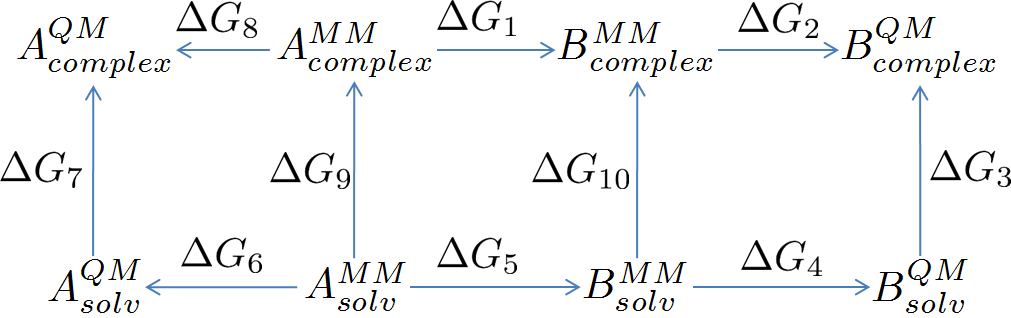
\includegraphics[width=15cm]{extended_thermodynamic_cycle.png}
 \captionof{figure}{The extended thermodynamic cycle}\label{fig:extended_thermodynamic_cycle}
\end{center}  

In this cycle, $\Delta G_1$ and $\Delta G_5$ are classical alchemical mutations of the ligand when bound in a protein and when in solvent respectively.  $\Delta G_2$, $\Delta G_4$, $\Delta G_6$ and $\Delta G_8$ are the perturbations from a classical system to a quantum system.  $\Delta G_7$ and $\Delta G_3$ are the desired free energies, but are much too computationally expensive to calculate.  However, with all the other free energies, the relative free energy ($\Delta G_7-\Delta G_3$) can be calculated by $\Delta G_1 + \Delta G_2 - \Delta G_4 - \Delta G_5 + \Delta G_6 - \Delta G_8$.

Application of the extended thermodynamic cycle has seen many uses, from reaction mechanisms \cite{Warshel_free_energy_correction, ryde_qm-mm_extended_td} to correcting binding free energies \cite{essex_qmmm, fox_mm_to_qm, mullholland_qmmm}  For the purposes of this thesis, the application will be directed toward correcting binding free energies.  Beierlein et al. \cite{essex_qmmm} correct the binding free energy using the Coulomb energies in a single step perturbation from the classical potential to a QM/MM potential.  Fox et al. \cite{fox_mm_to_qm} performed a similar task on the solvation free energies using the interaction energies this time perturbing from the classical to a fully quantum potential.  In both studies the Zwanzig equation \cite{zwanzig} was used (equation \ref{eq:Zwanzig}), however, although convergence was achieved by using interaction energies, this equation requires the use of total energies.  

\begin{equation} \label{eq:Zwanzig}
\ \Delta G = -k_B T \ln \left\langle \exp \left[ - \frac{E_{MM} - E_{QM}}{k_B T}  \right] \right\rangle
\end{equation}

Where $E_{MM}$ is the classical potential energy and $E_{QM}$ is the quantum potential energy, when interaction energies are used, these become $\Delta E_{MM}$ and $\Delta E_{QM}$.  Interaction energies can simply be described by the following,

\begin{equation}
\ E= E_{complex}-E_{ligand}-E_{host} \\.
\end{equation}

This cancels out any intramolecular terms and intermolecular interactions within the host.  The complex is the entire system e.g. a ligand bound to a protein, and within this example the host would be the protein in the same geometry but without the ligand present.  This makes the approximation that this conformation of the protein would be sampled in the absence of the ligand.  Although an approximation, it is an approximation that can provide converged free energies \cite{essex_qmmm, fox_mm_to_qm}.  One potential issue of using total energies is the overlap of configurational space.  However, Woods et al. \cite{mullholland_qmmm} have come up with a method that allows the perturbation from a classical system to a QM/MM system with the use of total energies.  Doing this involved evaluating whether a classically obtained snapshot was a good representation at the QM/MM level and accepting or rejecting it.

The search for a method that can provide accurate free energies of binding that is relatively inexpensive is one of the main challenges within computational chemistry.  As such, within this thesis, we would like to explore the possibilities of finding a method that can accurately calculate quantum corrected free energies for a range of systems when using total energy approaches.


%Chapter 1 introduction?
%Fox et al. \cite{fox_MM_to_QM} provides a brief description of the issues associated with using total energies, namely that the large size difference between the classical and quantum energies makes the calculation of the exponential numerically unstable and that there may be an issue with convergence of free energies obtained when using total energies.  
\include{Results_ch_1/Results_ch_1}
%\include{Results_ch_2/Results_ch_2}
%\include{Results_ch_3/Results_ch_3}
%\include{Results_ch_4/Results_ch_4}
%\chapter{Conclusions} \label{Chapter:conclusions}

We have presented a way to correct classical binding energies and the steps leading up to the final method.  These steps have shown several important problems with quantum corrections.  Chapter XXX shows the issue of using a SSP approach to correcting free energies, namely that large ``jumps'' are present within the free energy.  These ``jumps' are as a result of energy outliers at the low energy tail of the energy difference distribution.  This distribution has a large range, even for the simple systems used within this Thesis.  If further examination is performed on the outliers within the energy difference distribution, it is found that they are not outliers in either the classical or quantum energy distributions.  However, they are on different sides of the distributions.  This highlights the inexact overlap of the configurational space.

The issue of inexact overlap was then further investigated by perturbing between two classical potentials with different charges.  It was found that by adjusting the overlap slightly the energy does not converge not only between runs, but the forward and reverse process too.  This showed the sensitivity of the Zwanzig equation and led to the examination of post-processing methods with an aim to ``smooth'' over the low energy tail.  First a Gaussian distribution was fitted to the energy difference.  Numerical integration showed much improved convergence on the direct SSP approach, but still yielded a difference of over 6 kcal/mol between runs.  Additionally an analytical approach was applied, which emphasized the sensitivity of the exponents on the convergence of the free energy.  Specifically, the variance or $\alpha$ exponent has the largest effect on the free energy.  Again this is due to the low energy tail of the distribution, by only allowing data from ten thousandth height of the Gaussian the free energy converges.  However, there is no scientific reason to ignore part of the data, which shows that no post-processing method can be applied to increase the convergence.  This led to the importance of finding an accurate representation of the QM configurational space.






The next steps for this project would be to apply the final method to a more real test system.  This should be much closer to a protein-ligand binding site, but much smaller, for example, cyclodextrin bound to a variety of small organic ligands.  This would provide a non-uniform polarity around the ligand and should show the real benefit this method can have on complex systems.
%\appendix
%\include{AppendixA}
\backmatter


\bibliography{mybib}
\bibliographystyle{unsrt}
\end{document}
%% ----------------------------------------------------------------
